%% \documentclass[handout,t]{beamer} % HANDOUT
%% \documentclass[handout,notes=show,t]{beamer} % NOTES
\documentclass[t]{beamer} % SLIDES
\usepackage{etex}

\usetheme{DSM}
\usepackage{beamer-tools-dsm}

%%
%% some useful macros: mathematical notation etc.
%%

%% abbreviations for logic symbols
\renewcommand{\implies}{\Rightarrow}
\newcommand{\equivalent}{\Leftrightarrow}

%% abbreviations for common number spaces
\newcommand{\setN}[1][]{\mathbb{N}_{#1}} % allows \setN and \setN[0]
\newcommand{\setZ}{\mathbb{Z}}
\newcommand{\setQ}{\mathbb{Q}}
\newcommand{\setR}{\mathbb{R}}

%% sets and (sub-)sets defined by condition
\newcommand{\set}[1]{\{#1\}}
\newcommand{\setdef}[2]{\set{#1\,|\,#2}}
\newcommand{\bigset}[1]{\bigl\{#1\bigr\}}
\newcommand{\bigsetdef}[2]{\bigset{#1\bigm|#2}}
\newcommand{\setscale}[1]{\left\{#1\right\}}
\newcommand{\setdefscale}[2]{\setscale{#1\left|\,#2\right.}}

%% absolute value and norm
\newcommand{\abs}[1]{\lvert #1\rvert}
\newcommand{\bigabs}[1]{\bigl\lvert #1\bigr\rvert}
\newcommand{\absscale}[1]{\left\lvert #1\right\rvert}
\newcommand{\norm}[2][]{\lVert #2\rVert_{#1}}
\newcommand{\bignorm}[2][]{\bigl\lVert #2\bigr\rVert_{#1}}
\newcommand{\normscale}[2][]{\left\lVert #2\right\rVert_{#1}}

%% complement set (with optional index)
\newcommand{\compl}[1][]{\mathcal{C}^{#1}}

%% power set: \powerset{\Sigma^*}
\newcommand{\powerset}[1]{\mathcal{P}(#1)}

%% uparrow: a \ua b = direct dominance in ordered tree
\newcommand{\ua}{\uparrow}

%% left-right arrow: this $\lra$ that
\newcommand{\lra}{\leftrightarrow}

%% expanded engineering notation: 4.2\x\e+5
\newcommand{\e}[2]{10^{\ifthenelse{\equal{#1}{+}}{}{#1}#2}}
\newcommand{\x}{\cdot}

%% arg max & min: \argmax_{x\in C}, \argmin_{x\in C}
\newcommand{\argmax}{\mathop{\text{arg~max}}}
\newcommand{\argmin}{\mathop{\text{arg~min}}}

%% infinitesimal elements: \dx, \dy = \dX{y}, \dz
\newcommand{\dX}[1]{\,\mathit{d{#1}}}
\newcommand{\dx}{\dX{x}}
\newcommand{\dy}{\dX{y}}
\newcommand{\dz}{\dX{z}}

%%% Local Variables: 
%%% mode: latex
%%% TeX-master: ""
%%% End: 
  % basic mathematical notation
%%
%% some macros for typesetting text
%%

%% \OPEN ... \CLOSE; \OPEN[np] ... \CLOSE[np]
%% bold large brackets for labelled bracketing notation
\newcommand<>{\OPEN}[1][]{\only#2{$\boldsymbol{\bigl[}\text{}_{\text{\raisebox{-2pt}{\textsc{#1}}}}$}}
\newcommand<>{\CLOSE}[1][]{\only#2{$\text{}_{\text{\raisebox{-2pt}{\textsc{#1}}}}\boldsymbol{\bigr]}$}}

%% \textgap ("_" representing missing letter)
\newcommand{\textgap}{\mbox{\hspace{.4pt}\texttt{\bfseries\secondary{\textunderscore}}\hspace{.4pt}}}

%% \textstar, \textast (math \star and \ast symbols in text mode, with some extra spacing)
% \newcommand{\textstar}{$\mspace{.8mu}\star\mspace{.8mu}$}
% \newcommand{\textast}{$\ast$}

%% $\p{\ctext{abc}}$ (cited text in mathematical equations, e.g. n-gram probabilities)
\newcommand{\ctext}[1]{\text{\textcite{#1}}}

%% $\p{\btext{abc}}$ (normal black text even in coloured math environment)
\newcommand{\btext}[1]{\text{\foreground{#1}}} 

%% text subscripts and superscripts (can be used in math and text mode)
\newcommand{\tsup}[1]{\ensuremath{^{\text{#1}}}}
\newcommand{\tsub}[1]{\ensuremath{_{\text{#1}}}}

%%% Local Variables: 
%%% mode: latex
%%% TeX-master: ""
%%% End: 
  % some useful macros for plain text
%%
%% some useful macros: statistical notation
%%

%% \p{X=k};  \pC{X=k}{Y=l};  \bigp{X_i = k};   \pscale{\frac{Z}{S^2}};
%% probability P(X=k) and conditional probability P(X=k|Y=l), also with larger or scaled parentheses
%% \p[\theta]{X=k};  \pC[\text{interpolated}]{X=k}{Y=l};  ...
%% with optional subscripts (for model probability, null probability, etc.)
\newcommand{\p}[2][]{\mathop{\mathrm{Pr}_{#1}}(#2)}
\newcommand{\pscale}[2][]{\mathop{\mathrm{Pr}_{#1}}\!\left(#2\right)}
\newcommand{\bigp}[2][]{\mathop{\mathrm{Pr}_{#1}}\bigl(#2\bigr)}
\newcommand{\pC}[3][]{\p[#1]{#2\,|\,#3}} 
\newcommand{\pCscale}[3][]{\pscale[#1]{#2\left|\,#3\right.\!}} 
\newcommand{\bigpC}[3][]{\bigp[#1]{#2\!\bigm|\!#3}} 

%% \Exp{X};  \Var{X};  \Exp[0]{X};  \Var[0]{X};  
%% \bigExp{X}; \bigVar{X}; \Expscale{X};  \Varscale{X};
%% expectation E[X] and variance V[X], expectation and variance under null hypothesis, 
%% and variants with largeer or scaled brackets
\newcommand{\Exp}[2][]{\mathrm{E}_{#1}[#2]}
\newcommand{\Var}[2][]{\mathop{\mathrm{Var}}_{#1}[#2]}
\newcommand{\bigExp}[2][]{\mathrm{E}_{#1}\!\bigl[#2\bigr]}
\newcommand{\bigVar}[2][]{\mathop{\mathrm{Var}}_{#1}\bigl[#2\bigr]}
\newcommand{\Expscale}[2][]{\mathrm{E}_{#1}\left[#2\right]}
\newcommand{\Varscale}[2][]{\mathop{\mathrm{Var}}_{#1}\left[#2\right]}

%% \pihat = \hat{\pi}
%% sampling estimate for population probability \pi (may need fine-tuning)
\newcommand{\pihat}{\hat{\pi}}

%% \Entropy{X}, \Entropy{p}, \KL{p}{q}, \MI{X}{Y}
%% \bigEntropy{}, \Entropyscale{}, \bigKL{}{}, \KLscale{}{}, \bigMI{}{}, \MIscale{}{}
%% entropy, KL distance, conditional entropy and mutual information (with scaled variants)
\newcommand{\Entropy}[1]{H[{#1}]}
\newcommand{\bigEntropy}[1]{H\bigl[{#1}\bigr]}
\newcommand{\Entropyscale}[1]{H\left[{#1}\right]}
\newcommand{\KL}[2]{D({#1}\|{#2})}
\newcommand{\bigKL}[2]{D\bigl({#1}\bigm\|{#2}\bigr)}
\newcommand{\KLscale}[2]{D\left({#1}\left\|{#2}\right.\right)}
\newcommand{\MI}[2]{I[{#1};{#2}]}
\newcommand{\bigMI}[2]{I\bigl[{#1};{#2}\bigr]}
\newcommand{\MIscale}[2]{I\left[{#1};{#2}\right]}

%% \corr (correlation) and \cov (covariance) as mathop's
\newcommand{\corr}{\mathop{\mathrm{corr}}}
\newcommand{\cov}{\mathop{\mathrm{cov}}
}
%%% Local Variables: 
%%% mode: latex
%%% TeX-master: ""
%%% End: 
  % notation for probability theory and statistics
%%
%% convenience macros for linear algebra (vectors and matrices)
%%

%% \Vector[i]{x} ... vector variable with optional _superscript_ index in parentheses
%% \Vector[']{x} ... special case: ' superscript not enclosed in parentheses
%% \vx, \vy, \vz ... abbreviations for common vector names
\newcommand{\Vector}[2][]{\mathbf{#2}\ifthenelse{\equal{#1}{}}{}{^{(#1)}}}
\newcommand{\vx}[1][]{\Vector[#1]{x}}
\newcommand{\vy}[1][]{\Vector[#1]{y}}
\newcommand{\vz}[1][]{\Vector[#1]{z}}
\newcommand{\vu}[1][]{\Vector[#1]{u}}
\newcommand{\vv}[1][]{\Vector[#1]{v}}
\newcommand{\vw}[1][]{\Vector[#1]{w}}
\newcommand{\va}[1][]{\Vector[#1]{a}} % vectors of coefficients
\newcommand{\vb}[1][]{\Vector[#1]{b}} % for basis
\newcommand{\ve}[1][]{\Vector[#1]{e}} % for standard basis of R^n
\newcommand{\vm}[1][]{\Vector[#1]{m}} % row vectors of term-term matrix
\newcommand{\vn}[1][]{\Vector[#1]{n}} % normal vector
\newcommand{\vmu}[1][]{\Vector[#1]{\boldsymbol{\mu}}} % column vectors of term-term matrix
\newcommand{\vf}[1][]{\Vector[#1]{f}} % row vectors of term-context matrix
\newcommand{\vphi}[1][]{\Vector[#1]{\boldsymbol{\phi}}} % column vectors of term-context matrix
\newcommand{\vxi}[1][]{\Vector[#1]{\boldsymbol{\xi}}} % coordinate vector
\newcommand{\vnull}[1][]{\Vector[#1]{0}} % neutral element

%% \Span{\vb[1],\ldots,\vb[k]} ... span of set of vectors
%% \Rank{...} ... rank of set of vectors or matrix
%% \Det{...}, \det A ... determinant of a set of vectors / a matrix A
%% \Image{f}, \Kernel{f} ... image and kernel of a linear map
\newcommand{\Span}[1]{\mathop{\text{sp}}\left(#1\right)}
\newcommand{\Rank}[1]{\mathop{\text{rank}}\left(#1\right)}
\newcommand{\Det}[1]{\mathop{\text{Det}}\left(#1\right)}
%% \det is already defined in the standard library
\newcommand{\Image}[1]{\mathop{\text{Im}}\left(#1\right)}
\newcommand{\Kernel}[1]{\mathop{\text{Ker}}\left(#1\right)}

%% \dist[2]{\vx}{\vy} ... distance between two vectors (p-metric)
\newcommand{\dist}[3][]{d_{#1}\left(#2, #3\right)}
\newcommand{\bigdist}[3][]{d_{#1}\bigl(#2, #3\bigr)}

%% \sprod{\vu}{\vv} ... scalar product
\newcommand{\sprod}[2]{\left\langle #1, #2 \right\rangle}
\newcommand{\bigsprod}[2]{\bigl\langle #1, #2 \bigr\rangle}


%%% Local Variables: 
%%% mode: latex
%%% TeX-master: ""
%%% End: 
% convenience macros for vectors and matrices

%%%
%%% local configuration adjustments
%%%

%%% You can change pre-defined colours here, override built-in macros from the
%%% style definition and standard library, as well as define macros needed by
%%% all local documents.

%%% e.g. adjust counterpoint (dark green) for data projectors where greens are
%%% far too bright, as well as green component of light colour and pure green
%%% (of course, it's a better solution to adjust the gamma settings of your monitor)
%%
%% \definecolor{counterpoint}{rgb}{.1, .3, 0}
%% \definecolor{light}{rgb}{.45, .3, .55}
%% \definecolor{puregreen}{rgb}{0, .35, 0}

%% ----- extra packages we need to load

\usepackage{tikz}
\usepackage{alltt}              % code examples with nicely formatted comments
\usepackage{hieroglf}           % hieroglyph font for the archeology example
\usepackage{rotating}
\usepackage{multirow}
\usepackage[normalem]{ulem}
\usepackage{calc}

\usetikzlibrary{arrows.meta}
\usetikzlibrary{shadows}
\usetikzlibrary{matrix}
\usetikzlibrary{positioning}

%% ----- predefined TikZ styles

%% diagram:
%%   box[=colour]   ... shaded text box with drop shadow
%%   arrow[=colour] ... thick arrow between boxes
%%   ghost          ... invisible box (white)
\tikzstyle{diagram box}[secondary]=[
rectangle, rounded corners=1ex, inner sep=5pt, minimum height=4ex, minimum width=4ex,
thick, draw=#1, top color=#1!5!white, bottom color=#1!25!white, drop shadow]

\tikzstyle{diagram dark box}[secondary]=[
rectangle, rounded corners=1ex, inner sep=5pt, minimum height=4ex, minimum width=4ex,
thick, draw=#1, text=white, top color=#1!70!white, bottom color=#1, drop shadow]

\tikzstyle{diagram ghost}=[
rectangle, rounded corners=1ex, inner sep=5pt, minimum height=4ex, minimum width=4ex,
thick, draw=white, color=white]

\tikzstyle{diagram arrow}[secondary]=[
->, >={Latex[width=4pt, length=4pt]}, ultra thick, color=#1]

%% matrix: **EXPERIMENTAL**
%%   fixed matrix[=grid]  ... matrix with fixed distances between cells
%%   cell matrix[=size]   ... cells with fixed size (as long as contents fit)
%%   bmatrix[=margin]     ... bracketed matrix with margin adjustment (margin = cell margin)
%%   nmatrix[=matrix]     ... plain matrix, but use same margin adjustment as bmatrix
%%   cellbox[=colour]     ... draw cell node as coloured box (must be applied as node style)
%%   boxnodes[=colour]    ... draw all cell nodes in cellbox style
%%   debug matrix         ... show node and matrix frames
\tikzstyle{fixed matrix}[1cm]=[
row sep={#1,between origins}, column sep={#1,between origins}, nodes={anchor=base}]
\tikzstyle{bmatrix}[4pt]=[
left delimiter={[}, right delimiter={]}, inner sep=1pt, outer xsep=-#1, nodes={inner sep=#1}]
\tikzstyle{nmatrix}[4pt]=[
inner sep=1pt, nodes={inner sep=#1}] % without delimiters, but adjusted spacing
\tikzstyle{cell matrix}[5mm]=[
nodes={minimum size=#1, text depth={0.3 * #1}, text height={0.7 * #1}, inner sep=0pt, anchor=center}]
\tikzstyle{cellbox}[primary]=[
fill=#1!40!white, draw=#1, line width=1pt]
\tikzstyle{boxnodes}[primary]=[
nodes={cellbox=#1}]
\tikzstyle{debug matrix}=[nodes={draw=red, thin}, draw=green, thin]

%% hacked latex dots that can be scaled properly, with some vertical adjustment
%% \scaleDots[<raise>]{<factor>}{<dots-command>}
%% \scaleVdots[<factor>]  ...  \vdots scaled by <factor>
%% \scaleDdots[<factor>]  ...  \ddots scaled by <factor>
%% \scaleCdots[<factor>]  ...  \cdots scaled by <factor>
\newcommand{\scaleDots}[3][0ex]{\scalebox{#2}{\raisebox{#1}{\normalsize\ensuremath{#3}}}}
\newcommand{\scaleVdots}[1][1]{\scaleDots[-0.5ex]{#1}{\vdots}}
\newcommand{\scaleCdots}[1][1]{\scaleDots{#1}{\cdots}}
\newcommand{\scaleDdots}[1][1]{\scaleDots[-0.3ex]{#1}{\ddots}}

%% ----- general copyright message (authors may change between versions of the tutorial)
\newcommand{\dsmcopyright}{%
  Copyright \textcopyright\ 2009--2026 Evert, Lapesa, Lenci \& Baroni | 
  Licensed under CC-by-sa version 3.0}


%% ----- automatically show TOC reminder at beginning of each subsection
\AtBeginSubsection[]
{
  \begin{frame}
    \frametitle{Outline}
    \tableofcontents[current,currentsubsection]
  \end{frame}
}

%% ----- some useful macros for the SIGIL course

%% \begin{Rcode} .. \end{Rcode}
\newenvironment{Rcode}[1][]{%
  \setbeamercolor{block title}{fg=counterpoint,bg=counterpoint!15!white}%
  \setbeamercolor{block body}{bg=counterpoint!5!white}\small%
  \begin{block}{#1}\begin{alltt}\ungap[1]}{%
      \ungap[1]\end{alltt}\end{block}} % \end{alltt} ... to deconfuse emacs

%% use \sbox{\Rbox} ... \usebox{\Rbox} to insert arbitray latex into Rcode environment
\newsavebox{\Rbox}

%% > plot(x,y)      \REM{this produces a scatterplot}
\newcommand{\REM}[2][\small]{\textsf{#1\color{primary}\# #2}}

%% nice colour for R output: \begin{Rout} .. \end{Rout}
\newenvironment{Rout}[1][\footnotesize]{%
  \begin{footnotesize}#1\color{secondary}\bfseries}{%
    \color{black}\mdseries\end{footnotesize}}

%% symbols for centroid vector and singular value matrix 
%% \newcommand{\vmu}[1][]{\boldsymbol{\mu}\ifthenelse{\equal{#1}{}}{}{^{(#1)}}}
\newcommand{\Msigma}{\boldsymbol{\Sigma}}

%% rotated column labels for table (to fit long text into narrow columns
\newcommand{\rotLabel}[2][60]{\begin{rotate}{#1}#2\end{rotate}}

%% allow very long matrices for row vectors
\setcounter{MaxMatrixCols}{20}
 % local adjustments to configuration and macros

\newcommand{\POS}[2][secondary]{$_{\text{\color{#1}\tiny #2}}$}
\newcommand{\VERB}[1][secondary]{\POS[#1]{VERB}}
\newcommand{\ADJ}[1][secondary]{\POS[#1]{ADJ}}
\newcommand{\NOUN}[1][secondary]{\POS[#1]{NOUN}}
\newcommand{\PN}[1][secondary]{\POS[#1]{NAME}}

\newcommand{\First}{1\textsuperscript{st}\xspace}
\newcommand{\Second}{2\textsuperscript{nd}\xspace}

% \usepackage{caption}
% \captionsetup[figure]{labelformat=empty}

%%%%%%%%%%%%%%%%%%%%%%%%%%%%%%%%%%%%%%%%%%%%%%%%%%%%%%%%%%%%%%%%%%%%%% 
%% Titlepage

\title[DSM Tutorial -- Part 4]{Distributional Semantic Models}
\subtitle{Part 4: A linguistic perspective on DSMs}
\author[\textcopyright\ Evert/Lapesa/Lenci/Baroni]{%
  Stephanie Evert\inst{1}\\
  {\small with  Gabriella Lapesa\inst{2}, Alessandro Lenci\inst{3}, and Marco Baroni\inst{4}}}
\institute[CC-by-sa]{%
  \inst{1}Friedrich-Alexander-Universität Erlangen-Nürnberg, Germany\\
  \inst{2}Heinrich-Heine-Universität Düsseldorf \& GESIS, Germany\\
  \inst{3}University of Pisa, Italy\\
  \inst{4}ICREA / Universitat Pompeu Fabra Barcelona, Italy
}

\date[wordspace.collocations.de]{
  \href{http://wordspace.collocations.de/doku.php/course:start}{\primary{\small http://wordspace.collocations.de/doku.php/course:start}}\\
  \light{\tiny \dsmcopyright}}

\begin{document}

\showLogo
\frame{\titlepage}
\hideLogo

%%%%%%%%%%%%%%%%%%%%%%%%%%%%%%%%%%%%%%%%%%%%%%%%%%%%%%%%%%%%%%%%%%%%%% 

\section*{Outline}
\frame{ 
  \frametitle{Outline}
  \tableofcontents
}

%%%%%%%%%%%%%%%%%%%%%%%%%%%%%%%%%%%%%%%%%%%%%%%%%%%%%%%%%%%%%%%%%%%%%%
\section{Does evaluation tell us everything?}

%%%%%%%%%%%%%%%%%%%%%%%%%%%%%%%%%%%%%%%%%%
\subsection{A cautionary tale}

\begin{frame}
  \frametitle{The CogALex-V Shared Task}
  \framesubtitle{\citet{Santus:etc:16}}

  \ungap[1]
  \begin{itemize}
  \item Aim: better linguistic understanding of DS from identification of specific \h{semantic relations}
  \item Data: 747 target words with approx.\ 10 candidate relata each
    \begin{itemize}
    \item training set: 318 targets, 3054 word pairs
    \item test set: 429 targets, 4260 word pairs
    \end{itemize}
  \item<2-> Subtask 1: related \vs unrelated word pairs
    \begin{itemize}
    \item unrelated pairs are random fillers
    \item[\hand] relatively easy: $F_1$ = 79.0\% (best system) %\vs 77.8\% (Mach5, our system)
    \end{itemize}
  \item<3-> Subtask 2: distinguish between semantic relations
    \begin{itemize}
    \item \textsc{syn}: $w_2$ can be used with same meaning as $w_1$
    \item \textsc{ant}: $w_2$ can be used as the opposite of $w_1$
    \item \textsc{hyper}: $w_1$ is a kind of $w_2$
    \item \textsc{part\_of}: $w_1$ is a part of $w_2$
    \item \textsc{random}: no relation (random word + manual check)
    \item[\hand] relatively hard: $F_1$ = 44.5\% (best system: \secondary{deep learning}) % \vs 29.5\% (Mach5, our system)
    \end{itemize}
  \end{itemize}
\end{frame}

\begin{frame}
  \frametitle{Mach~5 at CogALex 2016}
  \framesubtitle{\citet{Evert:16a}}

  \begin{itemize}
  \item Mach~5 participated in the CogALex-V Shared Task as a traditional ``count'' (non-neural) DSM 
    \begin{itemize}
    \item 10-billion-word Web corpus \citep{Schaefer:Bildhauer:12}
    \item syntactic dependencies from C\&C parser \citep{Curran:Clark:Bos:07}
    \item 26.5k target words, up to 300k feature dimensions
    \item other parameters set according to \citet{Lapesa:Evert:14a}
    \end{itemize}
    \gap[0.5]
  \item Parameter optimization on training data (subtask 1)
    \gap[1]
  \item Machine learning on optimized representations (subtask 2)
    \begin{itemize}
    \item learns relevance weights for 600 latent SVD dimensions
    \item best results from combination of different SVD spaces
    \end{itemize}
    \gap[0.5]
  \item[\hand] Try it yourself: {\small \url{http://www.collocations.de/data/\#mach5}}
  \end{itemize}
\end{frame}

\begin{frame}
 \frametitle{Mach~5: Parameter optimization}

 \ungap[1]
 \begin{center}
   \only<beamer:1| handout:1>{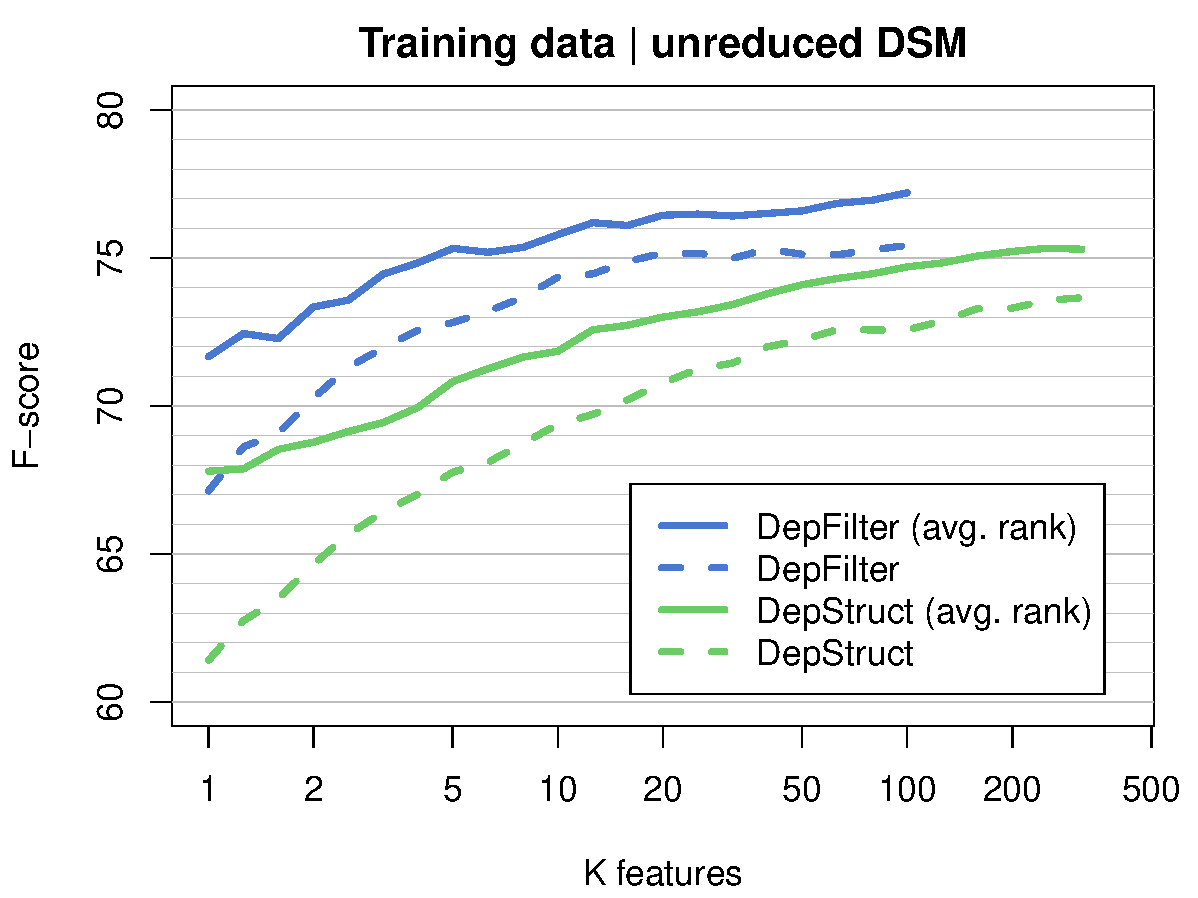
\includegraphics[width=9cm]{img/Mach5_eval_nfeat}}%
   \only<beamer:2| handout:0>{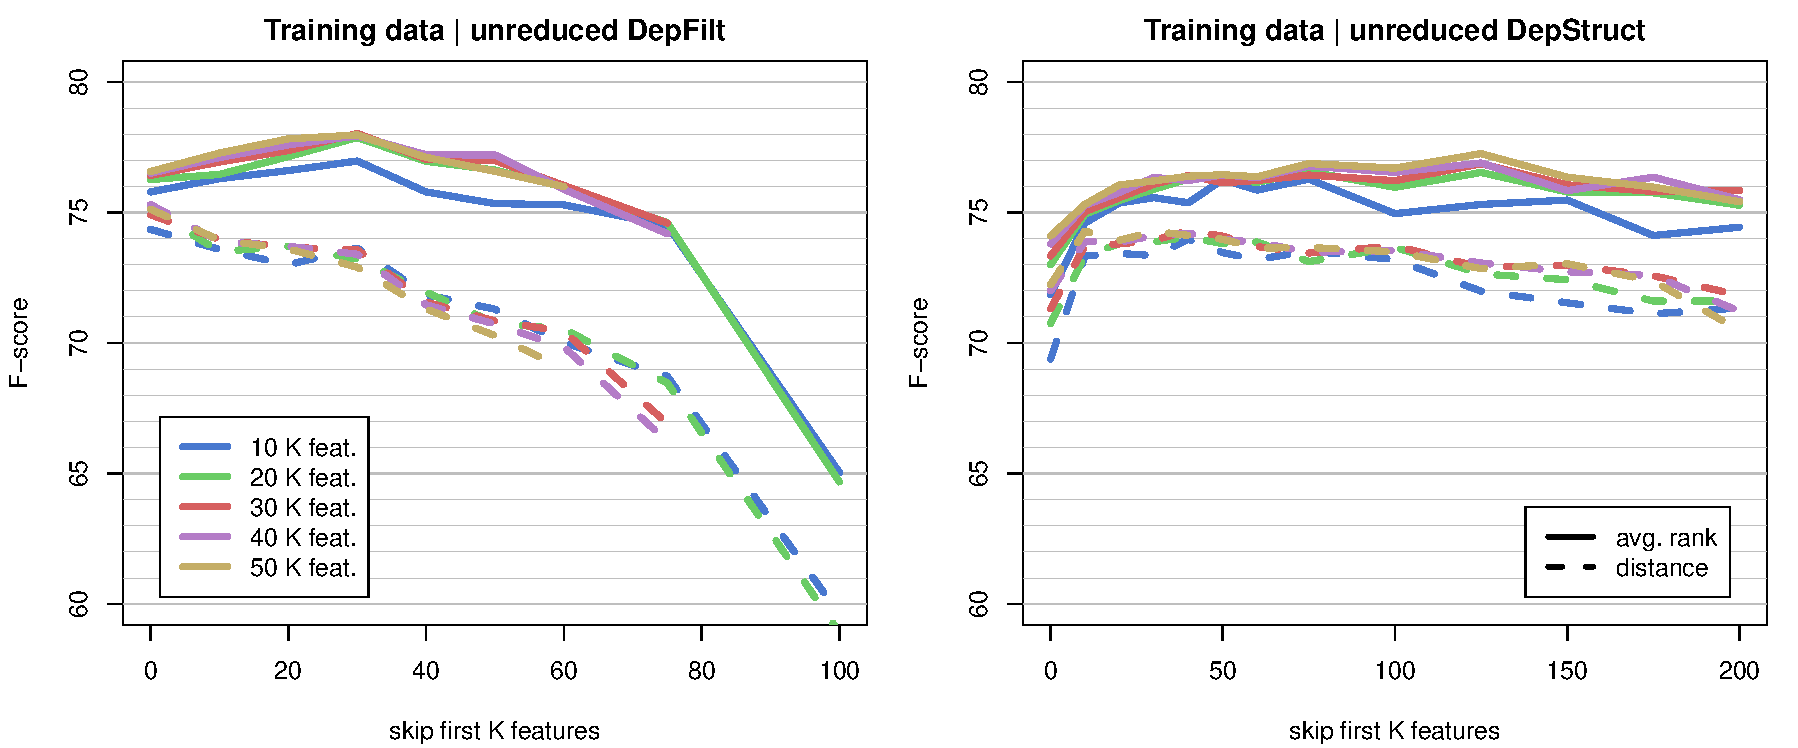
\includegraphics[width=9cm, trim={0 0 15.5cm 0}, clip]{img/Mach5_eval_features}}%
   \only<beamer:0| handout:2>{\hspace*{-1cm}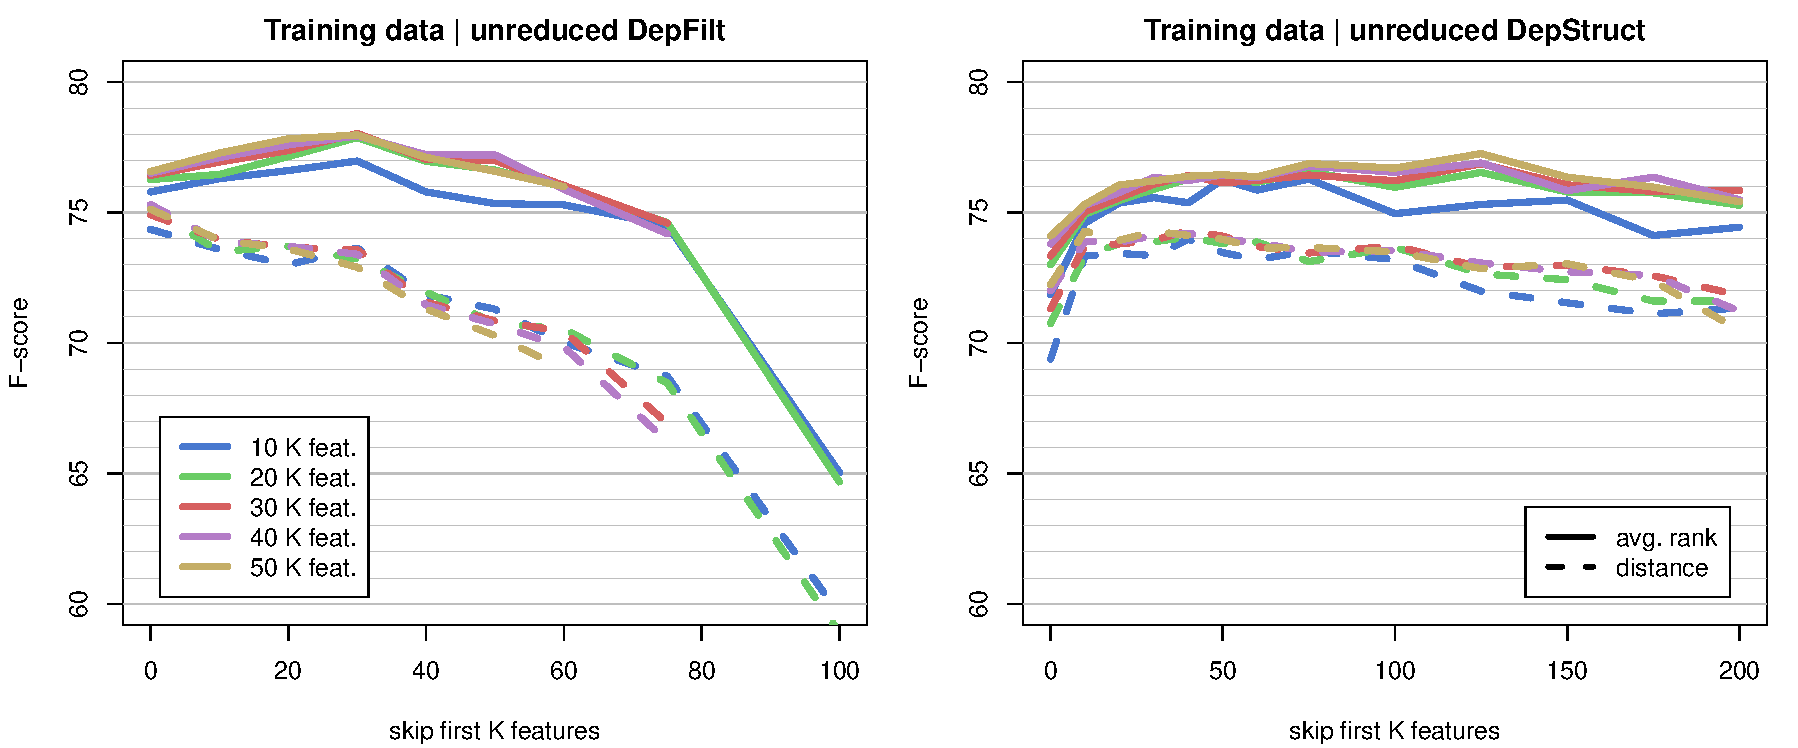
\includegraphics[width=12.5cm]{img/Mach5_eval_features}}%
   \only<beamer:3| handout:3>{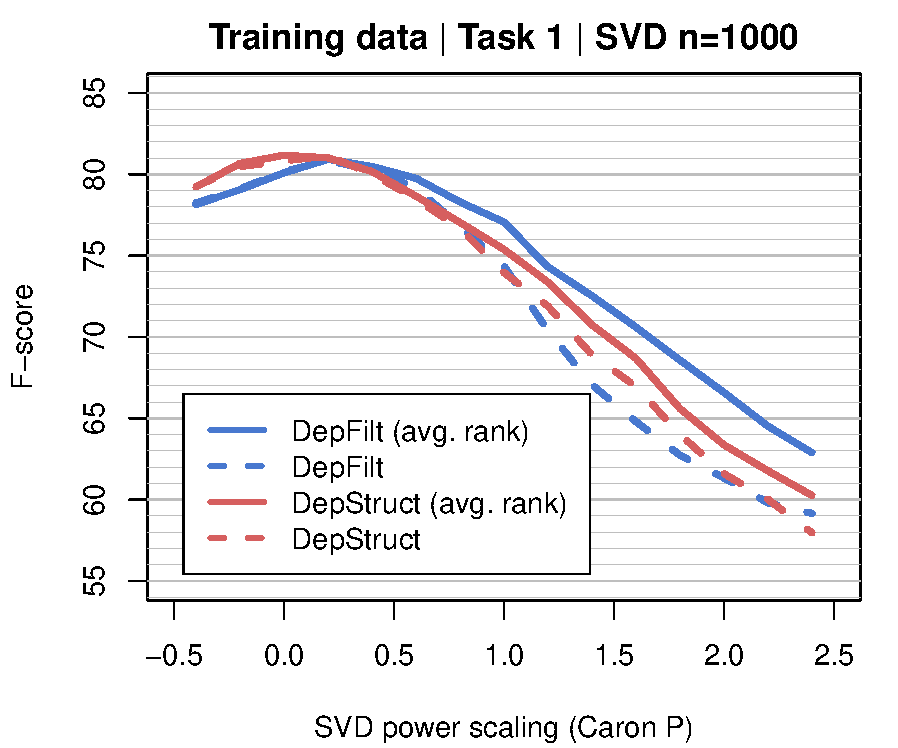
\includegraphics[width=9cm]{img/Mach5_eval_caron_P_task1}}%
   \only<beamer:0| handout:0>{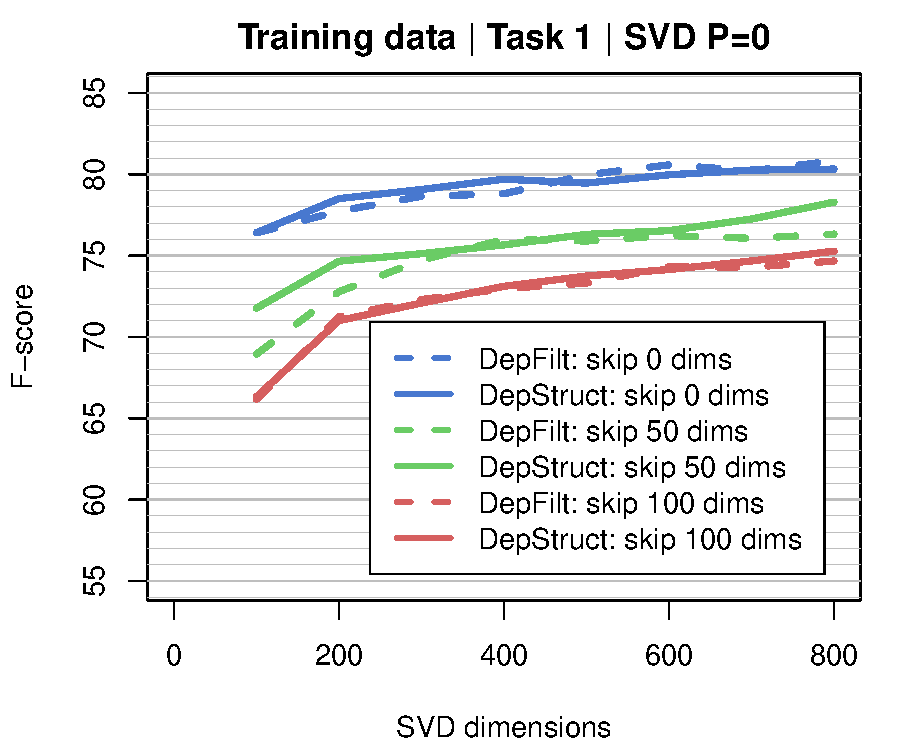
\includegraphics[width=9cm]{img/Mach5_eval_svd_dim_task1}}%
 \end{center}
\end{frame}

\begin{frame}
  \frametitle{Mach~5: Are we doing well?}
  
  \begin{center}
    \primary{$F_1 = 77.88\%$} for related \vs unrelated (best: 79.0\%)
  \end{center}

  However \ldots{}
  \begin{itemize}
  \item<2-> Parameter optimization yields surprising result:\\
    best model uses $<$ 50k features with relatively low frequency
    \gap
  \item<3-> Nearest neighbours are unsatisfactory, e.g.\ for \emph{play}:\\
    \emph{playing} ($54.1^{\circ}$), \emph{star} ($62.8^{\circ}$), \emph{reunite} ($62.9^{\circ}$), \emph{co-star} ($64.3^{\circ}$), \emph{reprise} ($64.4^{\circ}$), \emph{player} ($66.7^{\circ}$), \emph{score} ($68.5^{\circ}$), \emph{audition} ($69.2^{\circ}$), \emph{sing} ($69.4^{\circ}$), \emph{actor} (69.5), \emph{understudy} (69.6), \emph{game} (70.3), \ldots
    \gap
  \item<4-> Why is Mach~5 still doing so well in the task, then?  
  \end{itemize}
\end{frame}

\begin{frame}
  \frametitle{Mach~5: What is going wrong?}
  \framesubtitle{A disturbing result \ldots}

  \begin{center}
    \ungap[2]
    \only<beamer:1| handout:1>{%
      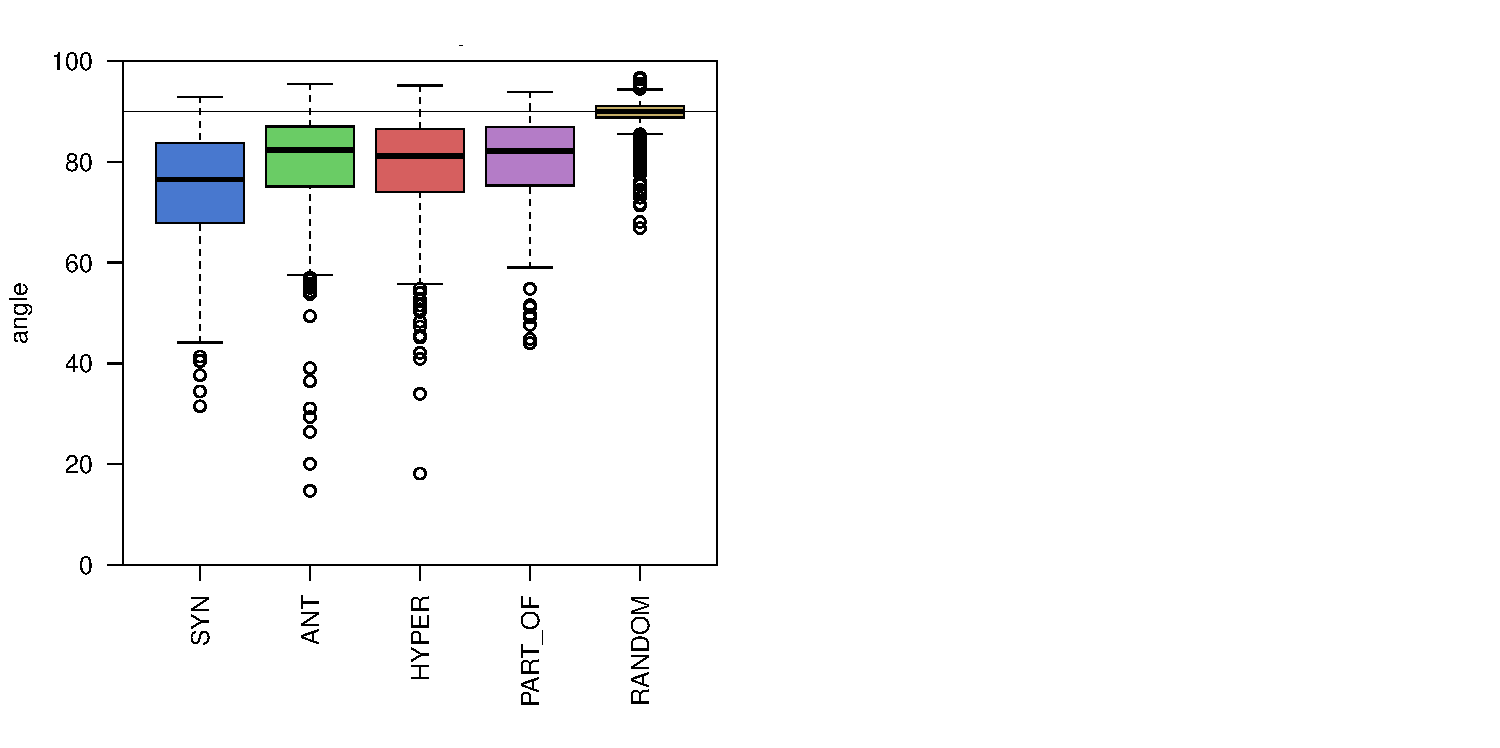
\includegraphics[width=7cm]{img/Mach5_boxplot_test_compare_left_panel}}%
    \only<beamer:2| handout:0>{%
      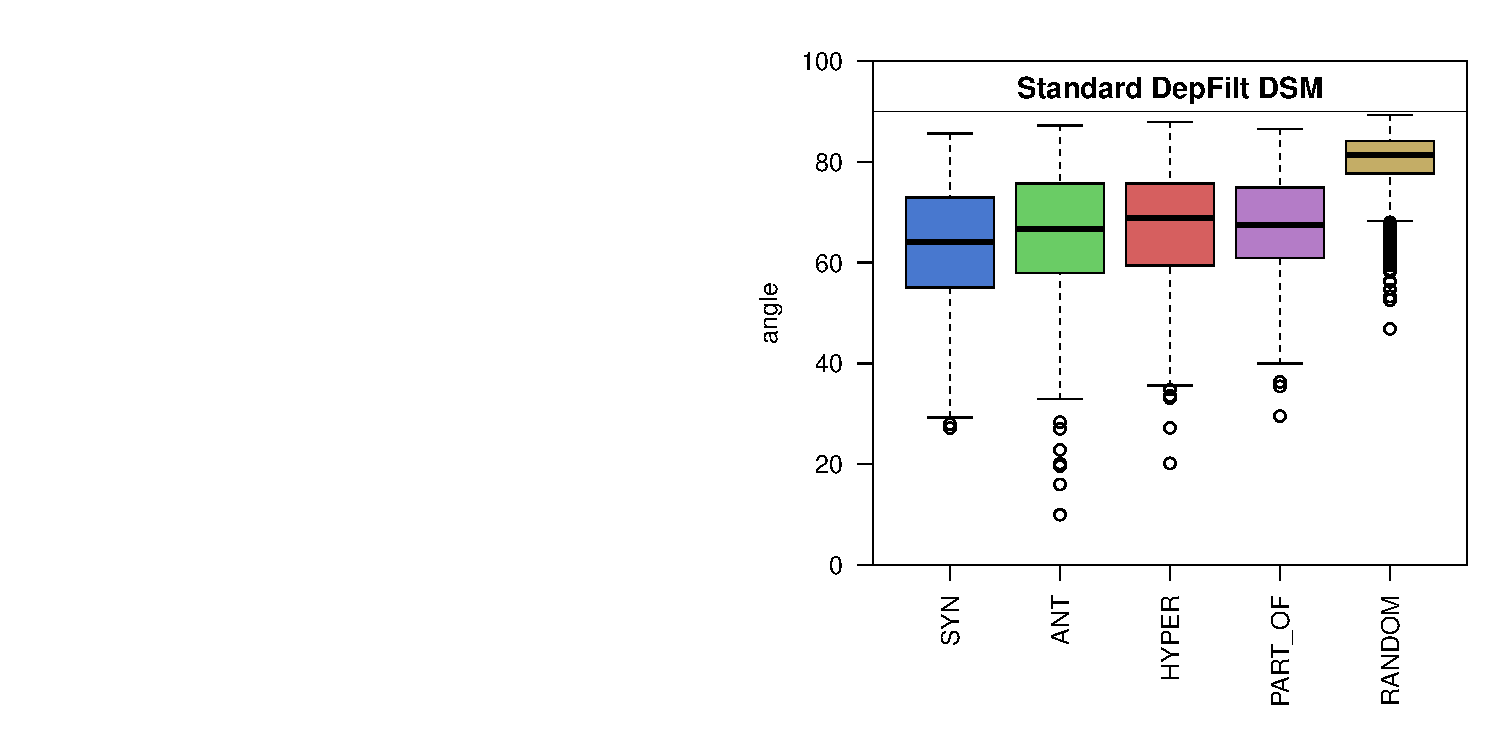
\includegraphics[width=7cm]{img/Mach5_boxplot_test_compare_right_panel}}%
  \end{center}
  \ungap[1]
  \begin{itemize}
  \item[\hand] DSM has learned to recognize random word pairs (at $90^{\circ}$)! 
  \item[\hand] We need better data sets with \hh{high-quality distractors}!
  \end{itemize}
\end{frame}

\begin{frame}
  \frametitle{Problems of standard tasks \& data sets}

  Problems with semantic interpretation of DSMs don't only stem from evaluation methodology \ldots\\
  \hfill \hh{\ldots{} data sets can be problematic as well!} 
  
  \gap[1]\onslide<2->
  Two major problems:
  \begin{itemize}
  \item DSMs may exploit contingent properties of the task
    \begin{itemize}
    \item \primary{random fillers} as distractors (``controls'')\\
      \So recognize random word pairs rather than semantic relations
    \item choice of clearly separated categories and prototypical exemplars in noun clustering task (ESSLLI 2008)\\
      \So much harder to identify categories in general word list
    \item typical superordinate-level words in hypernym detection task\\
      \So recognize ``typical hypernym'' in a multiple-choice setting
    \end{itemize}
    \gap
  \item Data set size too small
    \begin{itemize}
    \item e.g.\ 97.5\% accuracy on 80 TOEFL items \so over-fitting
    \end{itemize}
  \end{itemize}
\end{frame}


%%%%%%%%%%%%%%%%%%%%%%%%%%%%%%%%%%%%%%%%%%%%%%%%%%%%%%%%%%%%%%%%%%%%%%
\section{Beyond NLP: Linguistic evaluation}

\begin{frame}
  \frametitle{Outline}
  \tableofcontents[current]
\end{frame}

\begin{frame}
  \frametitle{DSM similarity \& linguistic theory}

  Numerical results from evaluation tasks can be misleading \ldots
  \begin{itemize}
  % \item also a serious problem in deep learning and LLM evaluation
  \item[\hand] \hh{perhaps a linguistic perspective gives us better insights?}
  \end{itemize}

  \vfill\onslide<2->
  \begin{enumerate}
  \item Polysemy
    \begin{itemize}
    \item a textbook challenge, will look at most intuitive solution 
    \item[\hand] hands-on: \code{hands\_on\_part4\_schuetze1998.R}
    \end{itemize}
  \item Compositionality
    \begin{itemize}
    \item above and below the word level
    \item[\hand] hands-on: derivational morphology \citep{Lazaridou:etc:13}
    \end{itemize}					
  \item Not all meaning is distributional
    \begin{itemize}
    \item e.g.\ function words, proper names
    \end{itemize}
  \item Distributional vectors as collocational profiles    
  \end{enumerate}

  \vfill\centering\onslide<3->
  Great overview paper:\\ \secondary{Distributional Semantics and Linguistic Theory} \citep{Boleda:20}	
\end{frame}
		

%%%%%%%%%%%%%%%%%%%%%%%%%%%%%%%%%%%%%%%%%%v
\subsection{Polysemy}		
		
\begin{frame}
  \frametitle{Polysemy in DSMs}

  \begin{itemize}
  \item \primary{Problem}: DSM vectors conflate contexts from different senses
    \begin{itemize}
    \item collocates of ``bank'': \emph{money}, \emph{river}, \emph{account}, \emph{swim}, \ldots
    \item conflated DSM vector either fits neither meaning well or is dominated by most frequent sense
    \end{itemize}
  \end{itemize}
  \pause
  % \begin{center}
  %   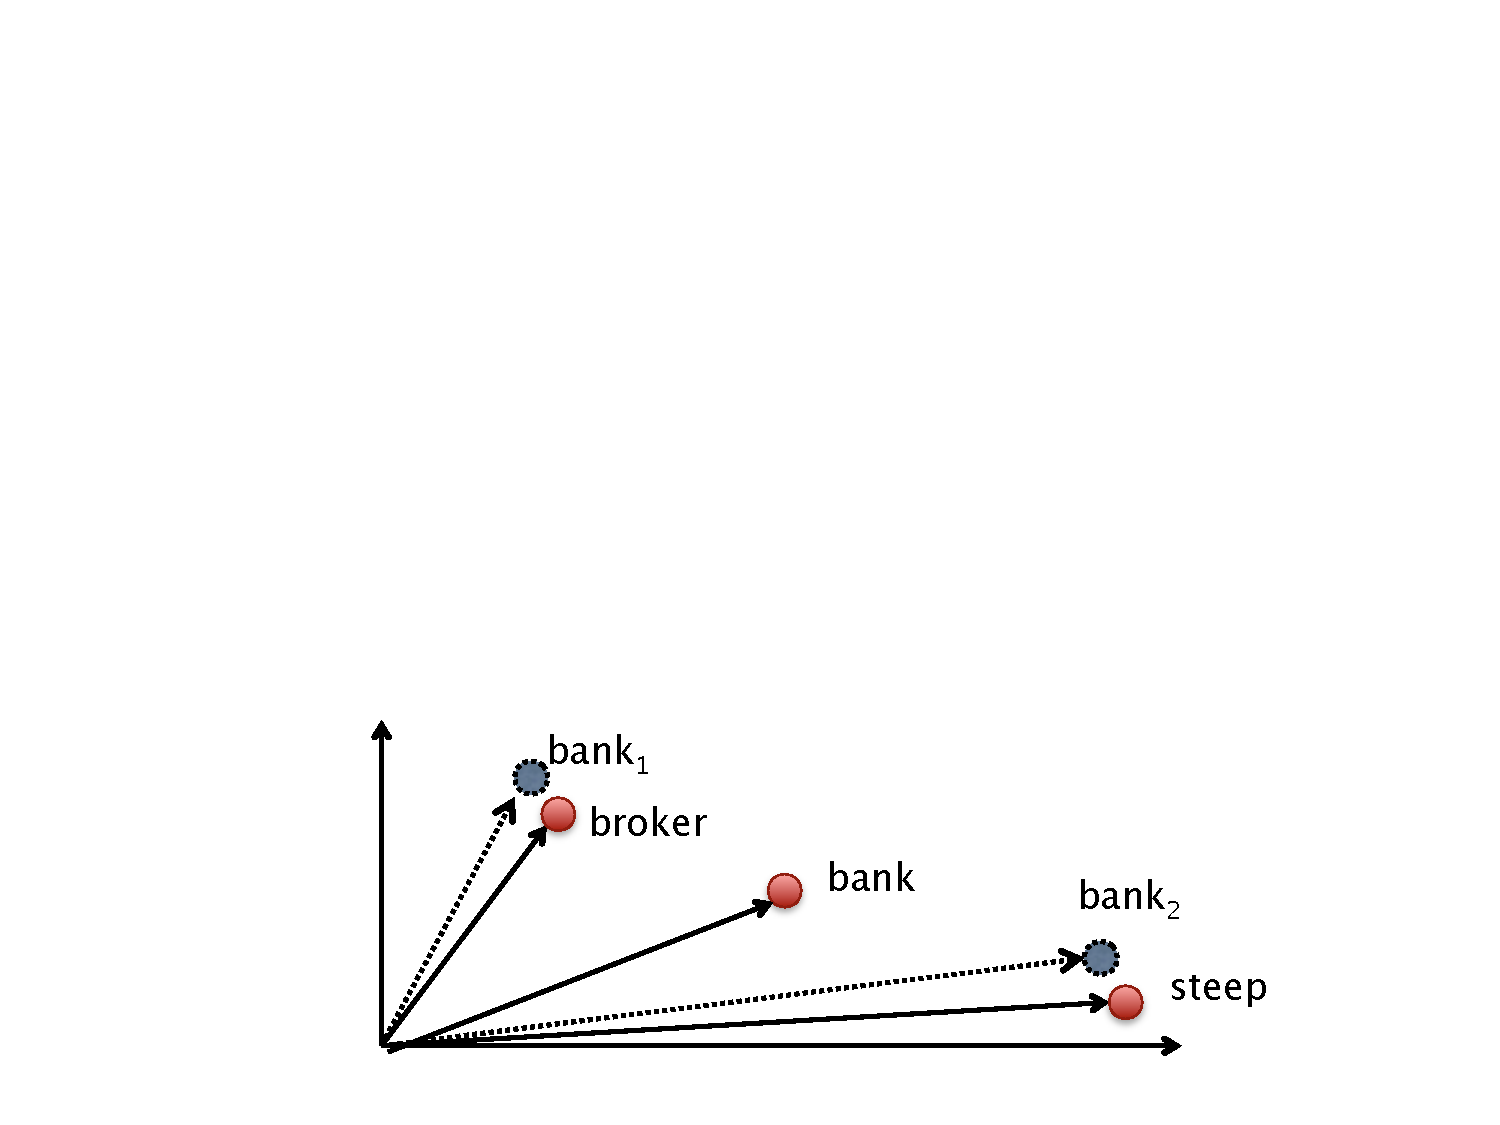
\includegraphics[scale=.6]{img/4_polysemy}
  % \end{center}

  \gap[1]
  \begin{center}
    \hspace*{-20pt}
    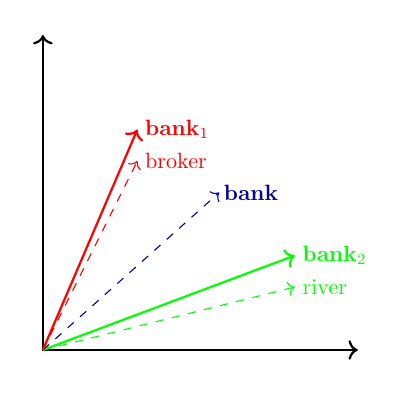
\begin{tikzpicture}[scale=0.8, every node/.style={transform shape}]
      \draw [<->, thick] (0,5) -- (0,0) -- (5,0);
      \node [left] at (0,5) {};
      \node [left] at (5,-0.3) {};
      \draw [->,thin, dashed,green] (0,0) -- (4,1);
      \draw [->,thick,green] (0,0) -- (4,1.5);
      \draw [->,thin, dashed,blue!60!black] (0,0) -- (2.8,2.5);
      \draw [->,thin, dashed,red] (0,0) -- (1.5,3);
      \draw [->,thick,red] (0,0) -- (1.5,3.5);

      \node [right,green] at (4,1) {river};
      \node [right,green] at (4,1.5) {\textbf{bank$_{2}$}};
      \node [right,red] at (1.5,3) {broker};
      \node [right,red] at (1.5, 3.5) {\textbf{bank$_{1}$}};
      \node [right,blue!60!black] at (2.75, 2.5) {\textbf{bank}};
    \end{tikzpicture}
  \end{center}
\end{frame}

\begin{frame}
  \frametitle{Polysemy in DSMs}
  \framesubtitle{Observation: DSM vectors conflate contexts from word senses}

  \begin{itemize}
  \item \primary{Solution}: build a representation for each instance of the word we want to disambiguate  \citep{Schuetze:98} \\
    \hfill \hand{} \primary{sentence vectors}
  \end{itemize}

  \begin{columns}
    \hspace*{35pt}
    \begin{column}{0.5\textwidth}
      \begin{block}{Target: bank} \footnotesize
        \textbf{bank$_{1}$}: \textit{The broker went to the bank to secure his cash} \\
        \textbf{bank$_{2}$}: \textit{The river bank was steep and dangerous}
      \end{block}
    \end{column} 
    \begin{column}{0.5 \textwidth}
      \begin{center}
        \hspace*{-25pt}
        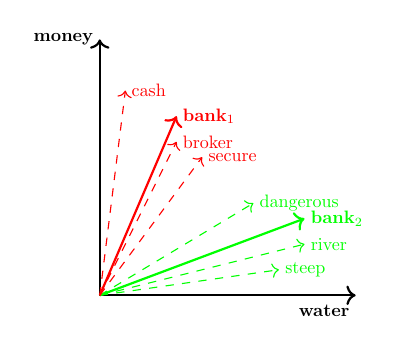
\begin{tikzpicture}[scale=0.65, every node/.style={transform shape}]
          \draw [<->, thick] (0,5) -- (0,0) -- (5,0);
          \node [left] at (0,5) {\textbf{money}};
          \node [left] at (5,-0.3) {\textbf{water}};
          \draw [->,thin, dashed,green] (0,0) -- (4,1);
          \draw [->,thin, dashed,green] (0,0) -- (3.5,0.5);
          \draw [->,thin, dashed,green] (0,0) -- (3,1.8);
          \draw [->,thick,green] (0,0) -- (4,1.5);

          \draw [->,thin, dashed,red] (0,0) -- (0.5, 4);
          \draw [->,thin, dashed,red] (0,0) -- (1.5,3);
          \draw [->,thin, dashed,red] (0,0) -- (2, 2.7);
          \draw [->,thick,red] (0,0) -- (1.5,3.5);

          \node [right,green] at (4,1) {river};
          \node [right,green] at (3.5,0.5) {steep};
          \node [right,green] at (3,1.8) {dangerous};
          \node [right,green] at (4,1.5) {\textbf{bank$_{2}$}};
          \node [right,red] at (2,2.7) {secure};
          \node [right,red] at (0.5,4) {cash};
          \node [right,red] at (1.5,3) {broker};
          \node [right,red] at (1.5, 3.5) {\textbf{bank$_{1}$}};
        \end{tikzpicture}\end{center}
    \end{column}
  \end{columns}

  \primary{Application: word sense disambiguation}\\
  \hfill \secondary{... can you think about another situation in which we may need it?}

\end{frame}

\begin{frame}[fragile]
  \frametitle{Context vectors: can we do them in \code{wordspace}?}
  \framesubtitle{Yes :--)}
  \ungap[1]
\begin{Rcode}
library(wordspace)
\REM{S1: ``Cats and dogs need their time'' }
s1 <- "cat and dog need their time" 
\REM{S2: ``Time is the cause not the effect'' }
s2 <- "time is the cause not the effect"
\REM{Ingredients: vectors for individual words }
>TT <- DSM_TermTermMatrix
>TT\begin{Rout}
       breed tail feed kill important explain likely
cat       84   17    8   38         0       2      0
dog      579   14   32   63         1       2      2
animal    45   11   86  136        13       5      4
time      19    8   29  134        94      44    100
reason     1    0    1   18        71     140     39
cause      0    1    0    3        55      35     51
effect     0    1    1    6        62      37     14
\end{Rout}
\end{Rcode}
\end{frame}

\begin{frame}[fragile]
\frametitle{Context vectors: can we do the, in \code{wordspace}?}
\framesubtitle{Yes :D}
\begin{Rcode}[``cats and dogs need their time'']
> context.vectors(TT, s1)\begin{Rout}
     breed tail feed     kill important explain likely
1 227.3333   13   23 78.33333  31.66667      16     34\end{Rout}
\REM{context.vectors() is taking the average of the values in each cell}
> (TT['cat','breed']+TT['dog','breed']+TT['time','breed'])/3 \begin{Rout}
227.3333\end{Rout}
\end{Rcode}
\begin{Rcode}[``time is the cause not the effect'']
round(context.vectors(TT, s2),3)\begin{Rout}
  breed  tail feed   kill important explain likely
1 6.333 3.333   10 47.667    70.333  38.667     55\end{Rout}
\end{Rcode}
\end{frame}


\begin{frame}[fragile]
  \frametitle{Context vectors: can we do them in \code{wordspace}?}
  \framesubtitle{Almost there \ldots}
  \ungap[1]
\begin{Rcode}
\REM{context.vectors() can also take a list as an input}
contexts <- round(context.vectors(TT, c(s1, s2)),2)
\REM{The output is a matrix, let's give it better rownames first}
rownames(contexts) <- c("s1", "s2") 
\REM{\ldots{} and then append it to our original matrix}
TT <- rbind(TT, contexts)
TT\begin{Rout}
        breed  tail feed   kill important explain likely
cat     84.00 17.00    8  38.00      0.00    2.00      0
dog    579.00 14.00   32  63.00      1.00    2.00      2
animal  45.00 11.00   86 136.00     13.00    5.00      4
time    19.00  8.00   29 134.00     94.00   44.00    100
reason   1.00  0.00    1  18.00     71.00  140.00     39
cause    0.00  1.00    0   3.00     55.00   35.00     51
effect   0.00  1.00    1   6.00     62.00   37.00     14
s1     227.33 13.00   23  78.33     31.67   16.00     34
s2       6.33  3.33   10  47.67     70.33   38.67     55
\end{Rout}
\end{Rcode}
\end{frame}

\begin{frame}[fragile]
  \frametitle{Context vectors: can we do them in \code{wordspace}?}
  \framesubtitle{And what now?}

\begin{Rcode}
\REM{We can do all the cool things we are used to do with DSM matrices}
\REM{Nearest neighbors...}
nearest.neighbours(TT, c("s1", "s2"), n=6)\begin{Rout}
$s1
     cat      dog   animal     time       s2    cause 
14.31016 17.16200 55.27587 62.66470 67.81707 77.90557 

$s2
    time    cause   effect   reason   animal       s1 
18.85097 25.19348 31.51682 40.83768 60.61621 67.81707 
\end{Rout}
\end{Rcode}
\end{frame}

\begin{frame}[fragile]
  \frametitle{Context vectors: can we do them in \code{wordspace}?}

  \ungap[1]
\begin{Rcode}
\REM{And a semantic map!}
plot(dist.matrix(TT))
\end{Rcode}

  \ungap[1]
  \begin{center}
    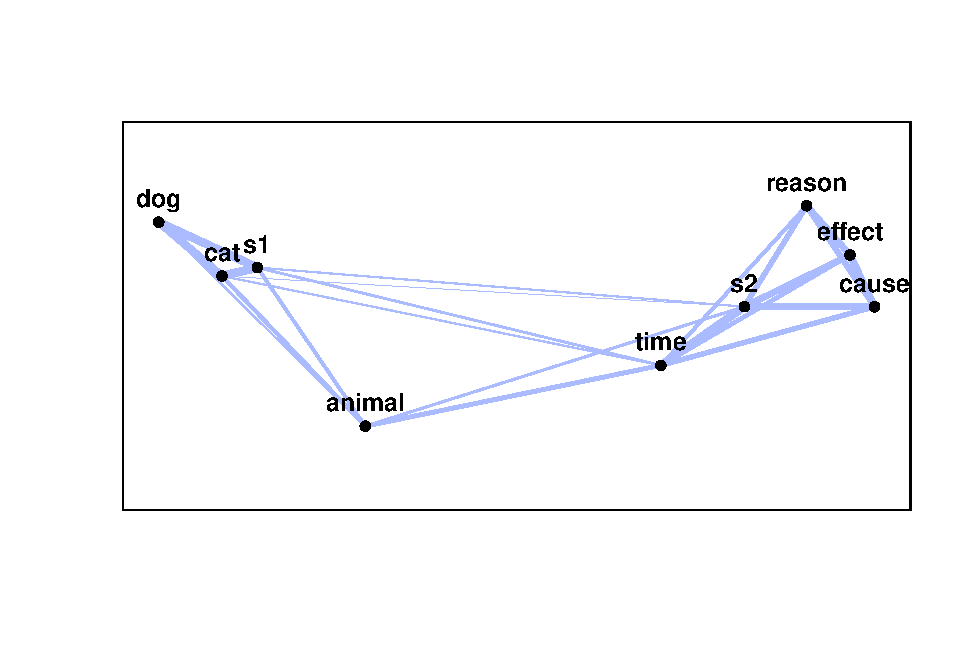
\includegraphics[scale=.50]{img/4_sem_map_cont}
  \end{center}

  \ungap[2.5]
  \begin{footnotesize}
    \primary{\texttt{hands\_on\_part4.R} also contains an example for \emph{bank}  with word2vec embeddings. If you enjoy centroids, try \texttt{hands\_on\_part4\_schuetze1998.R}!}
  \end{footnotesize}
\end{frame}


%%%%%%%%%%%%%%%%%%%%%%%%%%%%%%%%%%%%%%%%%% 
\subsection{Compositionality}

\begin{frame}
  \frametitle{Compositionality}
  \framesubtitle{Can we capture it in DS?}

  \begin{itemize}
  \item Formally: compositionality implies some operator \primary{$\bigoplus$}  such
    that 

    \begin{center}
      \primary{meaning(\primary{$w_1 w_2$}) = meaning(\primary{$w_1$})
        \primary{$\bigoplus$} meaning(\primary{$w_2$})}
    \end{center}

  \item{CDSM recipe}
    \begin{itemize}
    \item \primary{Distributional vectors} $\vv_1$ for $w_1$ and $\vv_2$ for $w_2$
    \item \primary{Operators}: mathematical stategies to combine $\vv_1$ and $\vv_2$ to \textit{predict} a vector representation $\vv_1 \oplus \vv_2$ for $w_1 w_2$
      \begin{itemize}
      \item vector addition
      \item vector multiplication
      \item nonlinear operations learned by neural networks
      \end{itemize}
    \end{itemize} 
  \item Problem: some words (e.g.\ \primary{\emph{not}}) are themselves more like  operators than points in space

    \vfill
    Great overview paper: \secondary{Frege in space: A program for compositional distributional semantics} \citep{Baroni:Bernardi:Zamparelli:14}	
  \end{itemize}
\end{frame}

\begin{frame}
  \frametitle{Compositionality with distributional vectors}
  \framesubtitle{Additive and Multiplicative Models \citep{Mitchell:Lapata:10}}

  % \begin{center}
  %   \begin{tabular}[c]{l|ccc}
  %     & \primary{practical} & \primary{difficulty} & \primary{problem} \\
  %     \hline
  %     \green{music} & 0 & 1 & 2 \\
  %     \green{solution} & 6 & 8 & 15 \\
  %     \green{economy} & 2 & 4 & 7 \\
  %     \green{craft} & 10 & 4 & 9 \\
  %     \green{create} & 4 & 0 & 1 \\
  %   \end{tabular}
  % \end{center}

  \begin{center}
    \begin{tabular}[c]{l|ccccc}
      & \primary{music} & \primary{solution} & \primary{economy}  &     \primary{craft}  &     \primary{create} \\
      \hline
      \secondary{practical} & 0 & 6 & 2 & 10 & 4 \\
      \secondary{difficulty} &1 & 8 & 4 & 4 & 0 \\
      \secondary{problem} & 2 & 15  & 7 & 9 & 1  \\
    \end{tabular}
  \end{center}

  \onslide<2->
  \begin{center}
    \primary{   {\large  $\vw = \vu + \vv$}}
  \end{center}
  \small{
    predicted(practical difficulty) = \textbf{practical} + \textbf{difficulty} = [1 14 6 14 4] }
  % predicted(practical difficulty) =\textbf{practical} + \textbf{difficulty} + \textbf{problem} = [3 29 13 23 5]
  
  \onslide<3->\gap[1]
  \begin{center}
    \primary{   {\large  $\vw = \vu \odot \vv$}}
  \end{center}
  \small{
    predicted(practical difficulty) = \textbf{practical} $\odot$ \textbf{difficulty} = [0 48 8 40 0] }

  \gap[1]
  \footnotesize{\secondary{What is your intuition about the effect of multiplication? How is it different from addition? Have you already seen it as an ingredient of something else?}}
\end{frame}

%\begin{frame}
%\frametitle{Compositionality}
%  \framesubtitle{Adjective Noun Composition (Baroni et al, 2014)\footnote{\url{https://iris.unitn.it/retrieve/handle/11572/98426/28081/baroni_bernardi_zamparelli.pdf}}}
%  \begin{center}
%   \includegraphics[scale=.40]{img/images/addmult} 
%  \includegraphics[scale=.20]{img/images/frege2}
%\end{center}
%\end{frame}

\begin{frame}
  \frametitle{How do I know my compositional vectors are ``good''?}
  \framesubtitle{Evaluation, again :)}

  \begin{enumerate}
  \item \hh{Qualitative inspection} of nearest neighbors of $\vu \oplus \vv$
    \begin{itemize}
    \item In which case look the neighbours intuitively more sensible?
    \item \emph{problem} would be ``good'' neighbour of practical \primary{$\oplus$} difficulty
    \item[]
    \end{itemize}
    
  \item<2-> \hh{Quantitative evaluation}
    \begin{itemize}
    \item Collect DSM vector for \emph{practical difficulty} in the same corpus\\[4pt]
    \item Evaluation criterion:\\
      observed(practical difficulty) $\approx$ predicted(practical difficulty)
      \begin{itemize}
      \item Would you expect \primary{+} or \primary{$\odot$} to work better?
      \end{itemize}
    \item Evaluation metric
      \begin{itemize}
      \item distance(predicted, observed) \citep{Lazaridou:etc:13}
      \item neighbour rank \citep{Baroni:Zamparelli:10,Pado:etc:16}
      \end{itemize}
    \end{itemize}
  \end{enumerate}
\end{frame}

\begin{frame}
\frametitle{How do I know my compositional vectors are ``good''?}
\framesubtitle{Observed \vs predicted vector}

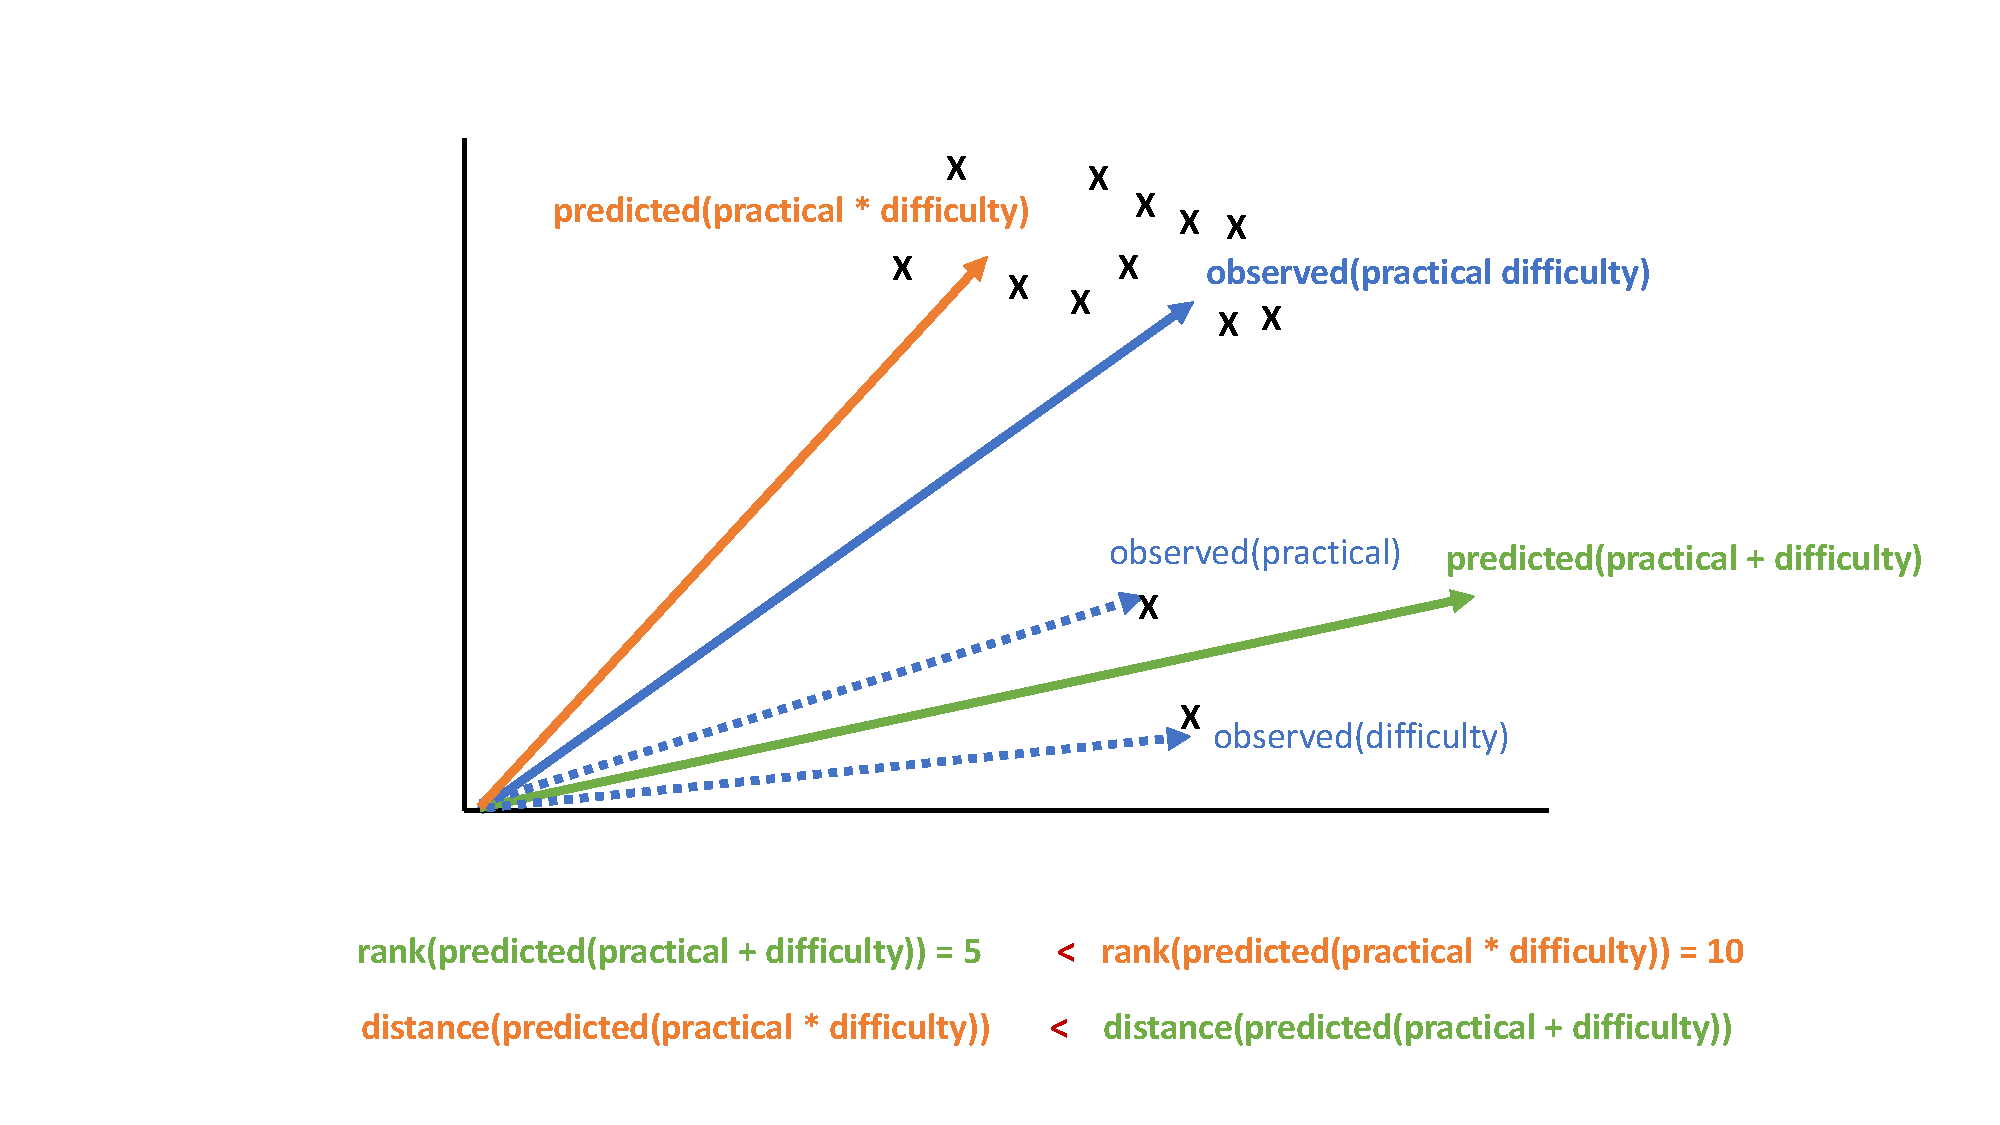
\includegraphics[scale=0.4]{img/4_eval_comp}
\end{frame}

\begin{frame}
  \frametitle{Adjective-noun composition \citep{Baroni:Zamparelli:10}}
  \framesubtitle{Starting point: observed AN vectors}

  \begin{itemize}
  \item Input: triples of \{observed(AN), A, N\}
    \begin{itemize}
    \item \{bad luck, bad, luck\}, \{red cover, red, cover\}, etc.
    \item 36 adjectives  (size, color, temporal, etc.)
    \end{itemize}
    \begin{center}
      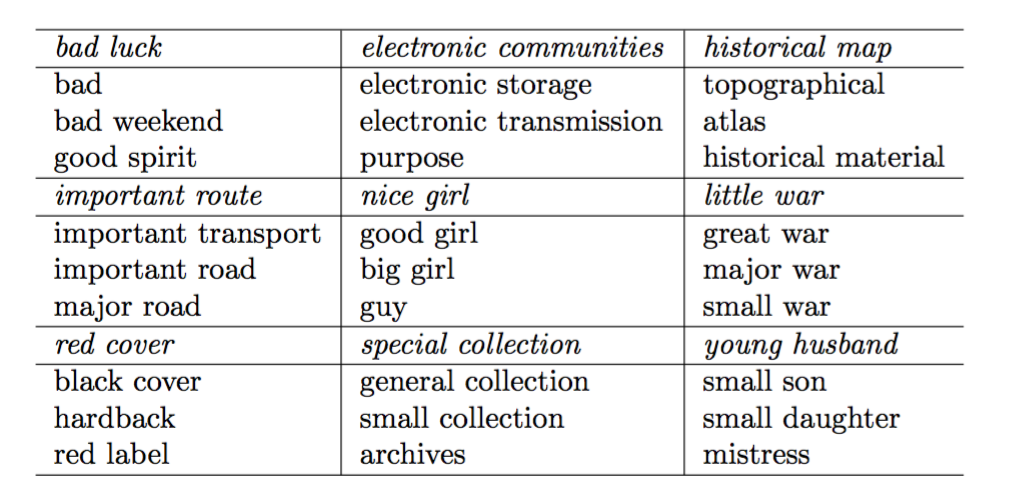
\includegraphics[scale=.40]{img/4_AN_observed} 
    \end{center} 	
  \item Methods: increasing computational complexity
    \begin{itemize} 
    \item unsupervised (additive, multiplicative) 
    \item[\hand] \secondary{supervised: learns matrix A by comparing AN and N}
    \end{itemize} 
  \end{itemize}
\end{frame}

\begin{frame}
  \frametitle{Adjective-noun composition \citep{Baroni:Zamparelli:10}}
  \framesubtitle{Observed(AN) \vs predicted(AN): neighbours}

  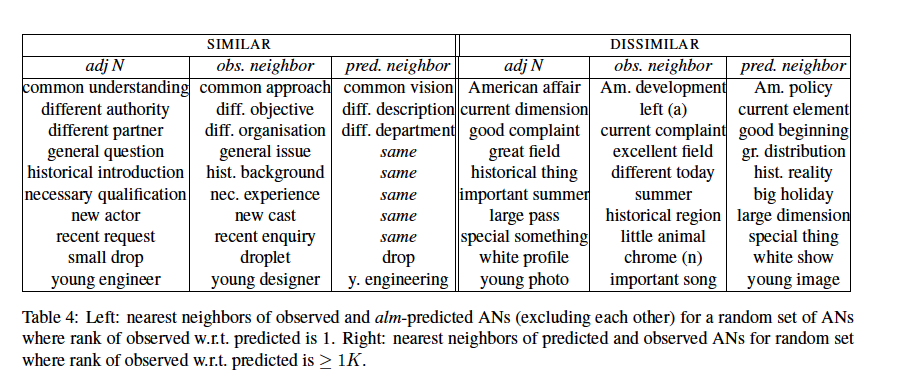
\includegraphics[scale=.70]{img/4_baroni_zamparelli_caption}
\end{frame}

\begin{frame}
  \frametitle{How about unattested AN combinations?}
  \framesubtitle{Capturing semantically deviant AN combinations \citep{Vecchi:etc:17}}

  \ungap[1]
  \begin{center}
    \hh{Can we use compositional DSMs to tell, among equally unattested AN, which one is semantically less plausible?}
  \end{center}
  \smallskip
  The \textit{composed vectors} for semantically deviant combinations (human ratings) will be \primary{farther away} from the head noun than the acceptable ones
  \begin{center}
    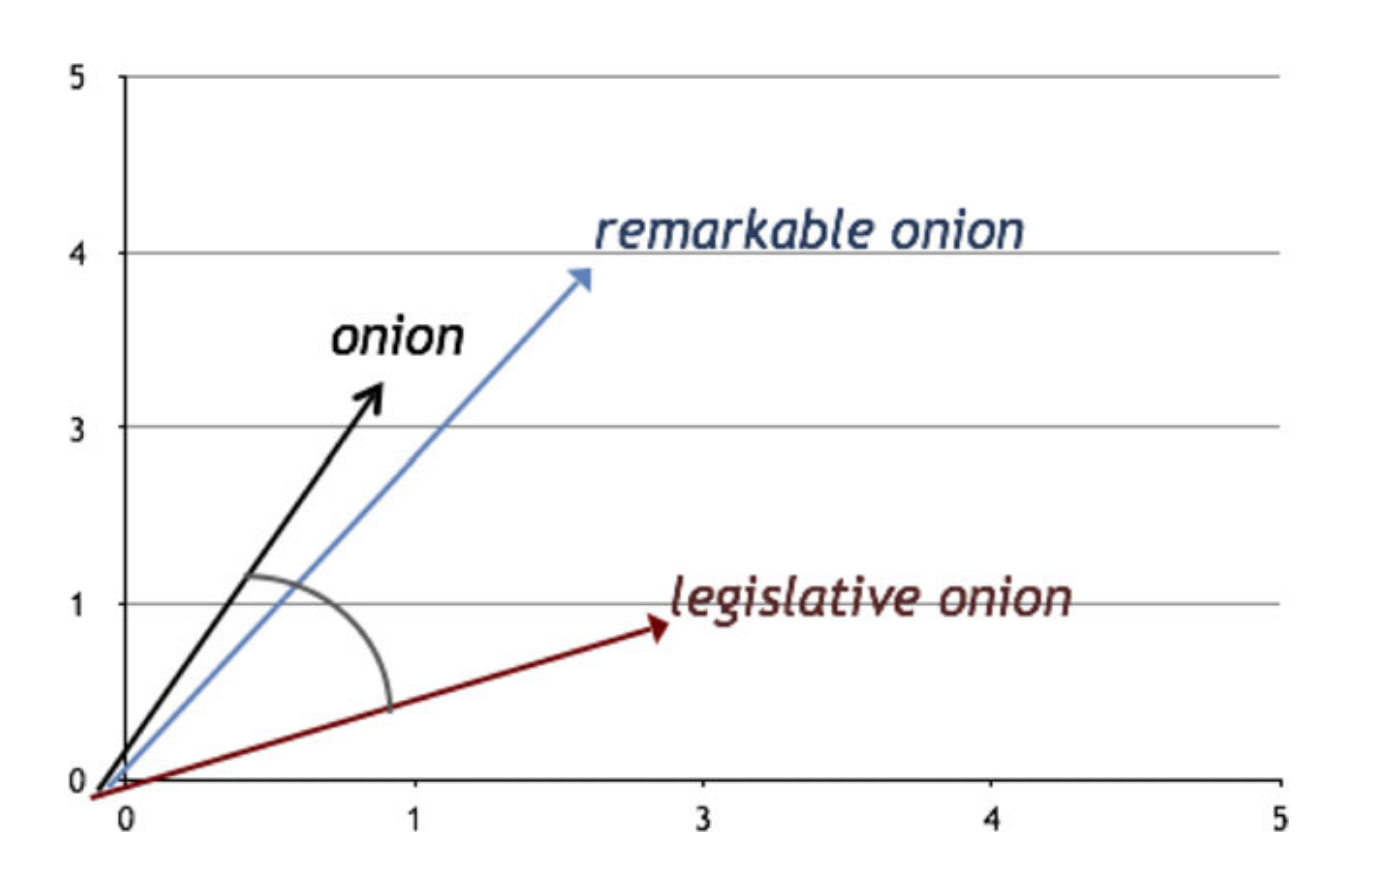
\includegraphics[scale=.2]{img/4_semdev}
  \end{center}
  \footnotesize
  ... they test other measures (e.g., neighbors density, vector length) as well as different composition methods: have a look at the paper!
\end{frame}

\begin{frame}
\frametitle{How about unattested AN combinations?}
  \framesubtitle{Capturing semantically deviant AN combinations \citep{Vecchi:etc:17}}

  \ungap[1]
  \begin{center}
    \hh{Can we use compositional DSMs to tell, among equally unattested AN, which one is semantically less plausible?}
  \end{center}
  \smallskip
  \primary{Qualitative inspection:} the \textit{composed vectors} of semantically acceptable pairs have plausible nearest neighbors
  \begin{center}
    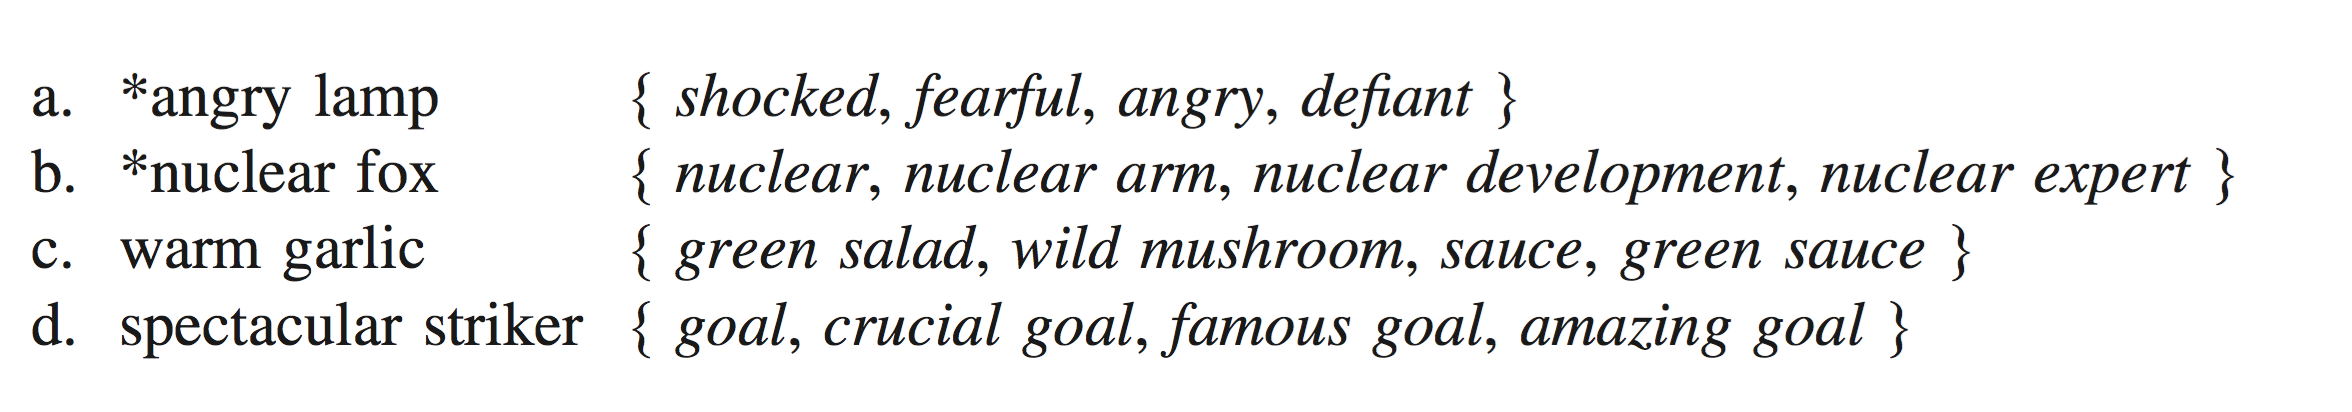
\includegraphics[width=\textwidth]{img/4_deviant}
  \end{center}
  
  \primary{\small\texttt{hands\_on\_part4.R} contains an implementation of vector addition and multiplication in \texttt{wordspace}. Have fun chasing the strangest AN combinations (and others as well)!}
\end{frame}

\begin{frame}
  \frametitle{Compositionality below the word level}
  \framesubtitle{Can we use compositional DSMs to investigate the meaning of derivational patterns?}

  \begin{columns}[c]
    \begin{column}{0.45\textwidth}
      \begin{center}
        \begin{tikzpicture}[scale=0.7, every node/.style={transform shape}]
          \draw [<->, thick] (0,5.5) -- (0,0) -- (5.5,0);
          \draw [->,thick,purered] (0,0) -- (5,1);
          \draw [->,thick,pureblue] (0,0) -- (2,5);
          \draw [->,thick,pureblue] (0,0) -- (4,2);
          \draw [->,thick,purered] (0,0) -- (2.2,3);
          \draw [->,very thick,puregreen] (4,2) -- (5,1);
          \draw [->,very thick,puregreen] (2,5) -- (2.2, 3);
          \node [right,purered] at (5,1) {hopeless};
          \node [right,pureblue] at (2,5) {happy};
          \node [right,pureblue] at (4,2) {hope};
          \node [right,purered] at (2.2,3) {unhappy};
          \node [right,puregreen] at (4.5,1.5) {\textbf{-LESS}};
          \node [right,puregreen] at (2.2,4) {\textbf{UN-}};
          \node [left,black] at (0,5.5) {\textbf{smile}};
          \node [below,black] at (5.5,0) {\textbf{people}};
        \end{tikzpicture}
      \end{center}
    \end{column}
    \begin{column}{0.55\textwidth}
      \begin{itemize}
      \item Starting point: vectors for \textcolor{pureblue}{base} and \textcolor{purered}{derived} words. 
      \item Two strategies:
        \begin{itemize}
 	\item[\hand] learn the \hh{semantic shifts} with compositional methods
 	\item investigate \hh{properties} of the \textcolor{puregreen}{patterns} $\rightarrow$ semantic relations%
	  \begin{itemize}
          \item zero-nominalisations as hyponyms of the base verb \citep{Varvara:Lapesa:Pado:21}
          \item \emph{un-} as antonyms of the base nouns	
          \end{itemize}	
        \end{itemize}
      \end{itemize}
    \end{column}
  \end{columns}
\end{frame}		

\begin{frame}
  \frametitle{The DS of Derivational Morphology \citep{Lazaridou:etc:13}}
  
  \begin{enumerate}
  \item Input: derived/stem vector pairs for each affix
    \begin{itemize}
    \item \emph{un-}: unfaithful/faithful, unbiased/biased, unwell/well
    \item \emph{-ly}: true/truly, mad/madly, deep/deeply
    \end{itemize}	
    \pause		
  \item Goal: \hh{build one representation per affix}
    \begin{itemize}
    \item No (well, little) learning (additive and multiplicative)
      \begin{itemize}
      \item \emph{un-} = centroid(unfaithful, unbiased, unwell, etc.) 
      \end{itemize}	
    \item Increasingly complex learning 
      \begin{itemize}
      \item parameters set during training to optimize composition, affixes as matrices (cf. adjectives)
      \end{itemize}
    \end{itemize}
    \pause				
  \item Prediction \& evaluation
    \begin{itemize}
    \item Apply affix to unseen base and compare predicted(derived) \vs observed(derived)
      \begin{itemize}
      \item simplest (additive) \& most complex (lexical functional, theoretically motivated): comparable
      \item cf.\ \citet{Pado:etc:16} for German: simple composition methods work better! 
      \end{itemize}
    \end{itemize}	
  \end{enumerate}			
\end{frame}

\begin{frame}
  \frametitle{The DS of Derivational Morphology \citep{Lazaridou:etc:13}}
  \framesubtitle{Dataset}

  \ungap[2]
  \begin{center}
    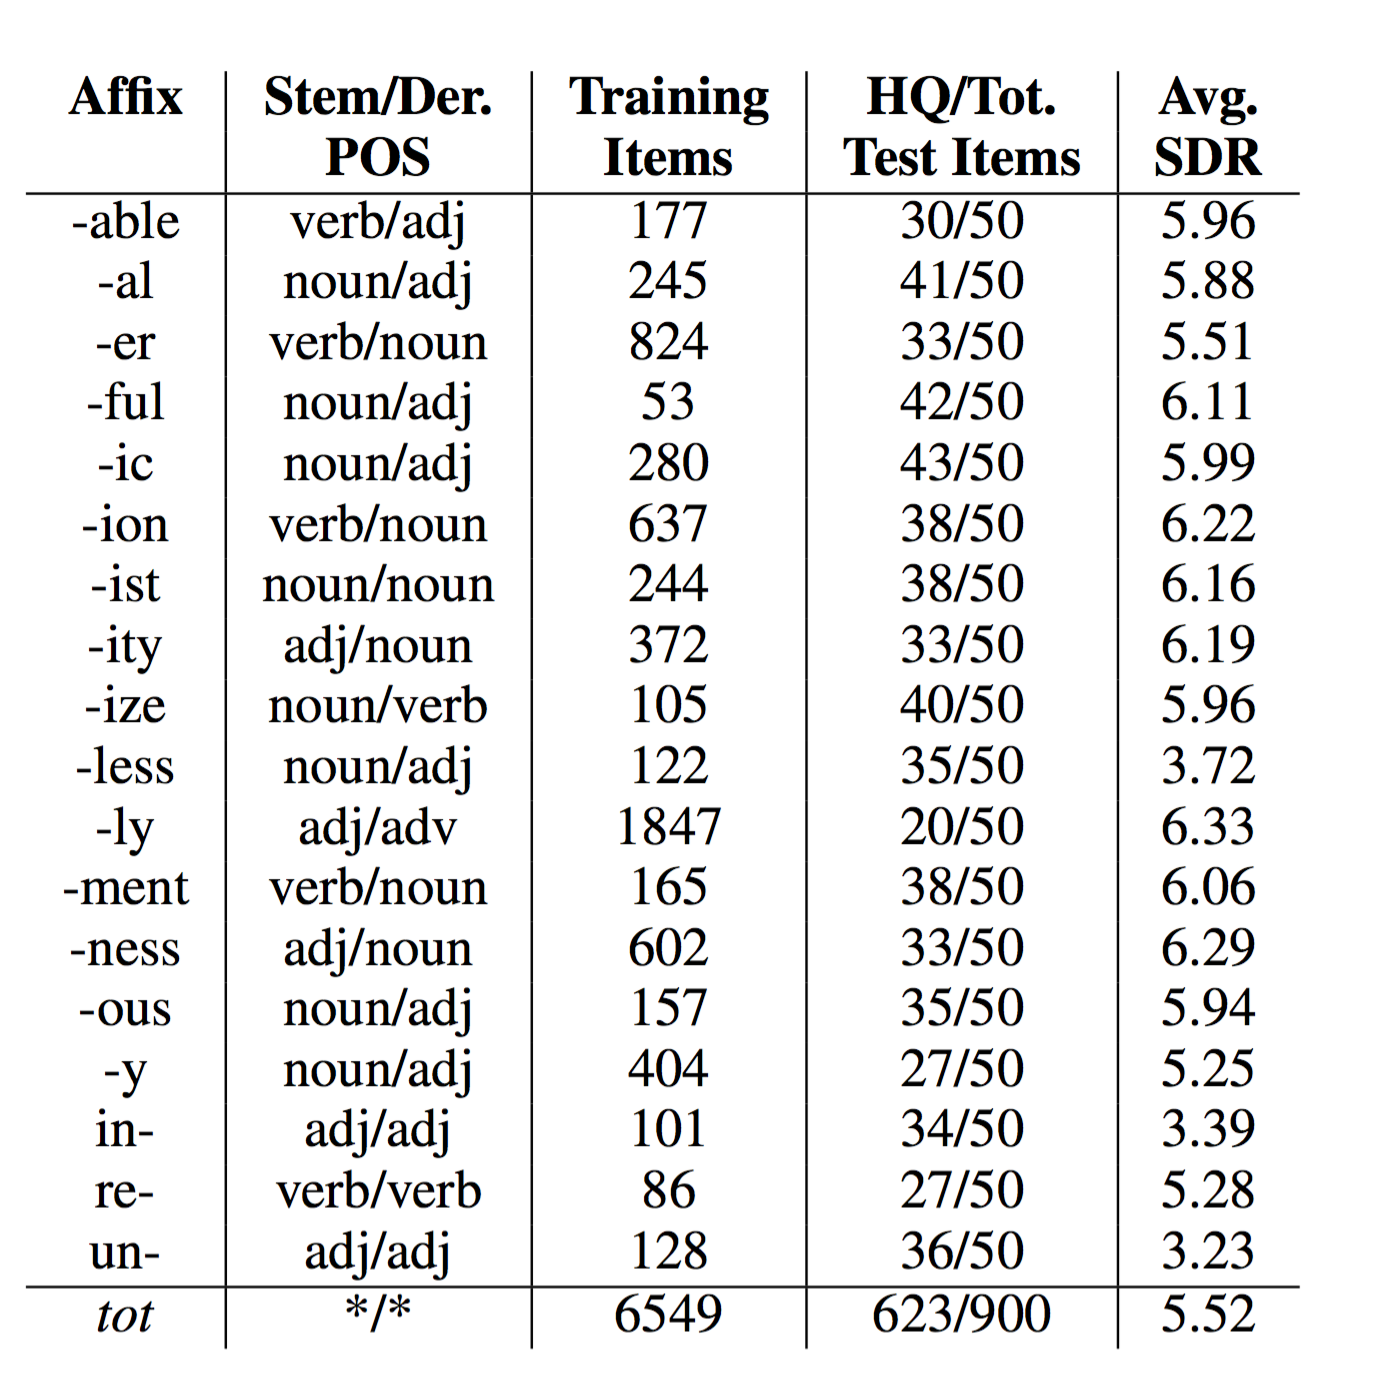
\includegraphics[scale=.25]{img/4_lazaridou_dataset} 
  \end{center}

  \footnotesize
  7000 base/derived pairs from CELEX, 18 patterns, training vs. test (further annotated for base/derived relatedness and vector quality)
\end{frame}	
		
%%%%%%%%%%%%%%%%%%%%%%%%%%%%%%%%%%%%%%%%%%
\subsection{Other linguistic aspects}		

\begin{frame}
  \frametitle{Not all semantic knowledge is distributional}

  \hh{Proper names} ``answer the purpose of \primary{showing} what thing it is that we are talking about but not of telling anything about it'' (Mill, 1843)
  \begin{itemize}
  \item Intuition: instances of categories such as PER, ORG, etc.
  \item \citet{Herbelot:15}, standard DSMs: category $\rightarrow$ instance
    \begin{itemize}\footnotesize
    \item ``\ldots{} upon encountering
      the name \textit{Mr Darcy} for the first time in the novel, a reader will attribute it the
      representation of the concept \textsc{man} and subsequently \primary{specialise} it as per the linguistic contexts in which the name appears''
    \end{itemize}			
  \item \citet{Westera:etc:21}, embeddings: instance $\rightarrow$ category
  \end{itemize}

  \onslide<2->\gap[1]
  \hh{Function words}: some pointers
  \begin{itemize}
  \item \citet{Baroni:etc:12} on quantifiers/entailment, \citet{Bernardi:etc:13} on determiners,  \citet{Pado:Hole:19} on the polysemy of the German reflexive \textit{sich}
  \end{itemize}
\end{frame}

\begin{frame}
  \frametitle{Making sense: collocational profiles \vs DSM vectors}
  \framesubtitle{Some exciting open questions for your consideration}
  
  \begin{itemize}
  \item For an unreduced term-term DSM, each row vector $\vm_t$ corresponds to the collocational profile of a target term $t$
    \begin{itemize}
    \item e.g.\ dependency-structured DSM \so word sketches
    \item[\hand] compare our own reading of sketch differences for nearest neighbours with distributional similarity
    \item[]
    \end{itemize}
  \item<2-> Can dim.-reduced vectors be read as collocational profiles?
    \begin{itemize}
    \item map to original features \so dense ``virtual'' collocational profile
    \item compare top-$k$ entries with original sparse profile
    \item[] 
    \end{itemize}
  \item<3-> Do DSM distances use the same information as the human interpretation of collocational profiles?
    \begin{itemize}
    \item humans likely to focus on few salient collocates, while DSM might exploit weak correlations across many dimensions
    \item cf.\ insights from authorship attribution \citep{Evert:etc:17}
    \end{itemize}
  \end{itemize}
\end{frame}

\begin{frame}
  \frametitle{Making sense: collocational profiles \vs DSM vectors}
  \framesubtitle{Some exciting open questions for your consideration}
  
  \begin{itemize}
  \item Can we figure out which features account for semantic differences?
    \begin{itemize}
    \item normalise vectors: $\norm{\vu} = \norm{\vv} = 1$
    \item $(u_i - v_i)^2$ = contribution to (squared) Euclidean distance
    \item for cosine similarity, contribution is $u_i v_i$
    \item[]
    \end{itemize}
  \item<2-> Collocations = \hh{first-order} association = \hh{syntagmatic}
  \item<2->  DSM similarity = \h{second-order} assocation = \h{paradigmatic}
    \begin{itemize}
    \item widely-held belief in distributional semantics, but is it true?
    \item some applications actually require both first-order and second-order assocation (e.g.\ \primary{free association norms})
    \item[\hand] we will obtain a few  mathematical insights in Part 5
    \item[]
    \end{itemize}
  \end{itemize}
\end{frame}


%%%%%%%%%%%%%%%%%%%%%%%%%%%%%%%%%%%%%%%%%%%%%%%%%%%%%%%%%%%%%%%%%%%%%%
\section{The FAST task}

%%%%%%%%%%%%%%%%%%%%%%%%%%%%%%%%%%%%%%%%%%
\subsection{Free association norms}

\begin{frame}
  \frametitle{Cognitive modelling with DSMs}

  \begin{itemize}
  \item \h{Why?} -- Because we want to know whether DS captures the mental lexical knowledge of human speakers!
    \gap
  \item<2-> Task: DSM predicts reaction times in \hh{priming experiments} \citep{Hare:etc:09,Lapesa:Evert:13}
    \begin{itemize}
    \item often just experimental items used for multiple-choice task \citep[e.g.][]{Pado:Lapata:07,Herdagdelen:Erk:Baroni:09}
    \item cf.\ tasks constructed from \code{Lazaridou2013} in previous section
    \item data sets of experimental items: \code{GEK\_Items}, \code{SPP\_Items}
    \end{itemize}
  \item<3-> Task: DSM predicts \hh{EEG potentials} \citep{Murphy:Baroni:Poesio:09} or \hh{fMRI brain activation} levels \citep{Mitchell:etc:08}
    \begin{itemize}
    \item huge datasets, but tiny and selective vocabulary
    \end{itemize}
  \item<4-> Task: DSM predicts human \h{free associations}
    \begin{itemize}
    \item often considered a ``window into the mental lexicon''
    \item free association norms available for thousands of cue words
    \end{itemize}
  \end{itemize}
\end{frame}

\begin{frame}
  \frametitle{Free associations}
  \framesubtitle{\ldots{} a cue into the organization of the mental lexicon?}

  \ungap[1]
  \begin{block}{\small Which words come to your mind if you hear \ldots}
    \begin{itemize}
    \item whisky $\rightarrow$ \visible<2->{gin, drink, scotch, bottle, soda}
    \item<2-> giraffe $\rightarrow$ \visible<3->{neck, animal, zoo, long, tall}
    \end{itemize}
  \end{block}
  \begin{itemize}	
  \item<4-> Hypotheses concerning the nature of the underlying process:
    \begin{itemize}
    \item Result of learning by contiguity \citep{James:90} \\
      \hfill \hand{} \primary{syntagmatic (\First-order)}
    \item Result of symbolic processes which make use of complex semantic structures \citep{Clark:70} 
      \hfill \hand{} \primary{paradigmatic (\Second-order)}
    \end{itemize}
  \item<5-> Large collections available 
    \begin{itemize}
    \item Edinburgh Associative Thesaurus (\hh{EAT})\\ \secondary{8210 stimuli, 100 subjects \citep{Kiss:etc:73}}
    \item University of South Florida Free Association Norms (\hh{USF})\\ \secondary{5019 stimuli, 6000 subjects \citep{Nelson:McEvoy:Schreiber:04}}
    \end{itemize}		
  \end{itemize}
\end{frame}

\begin{frame}
  \frametitle{Syntagmatic \vs paradigmatic relations}
  \framesubtitle{Definitions and general assumptions}

  \ungap[1]
  \begin{itemize}
  \item<1-> \hh{Syntagmatic} $\iff$ contiguity
    \begin{itemize}
    \item Examples: \{\textit{dog, barks}\}, \{\textit{dog, bone}\}
    \item Words appear together: \First-order co-occurrence
    \item Found in: collocational profiles, DSM dimensions
    \item[]
    \end{itemize}
  \item<2-> \hh{Paradigmatic} $\iff$ interchangeability 
    \begin{itemize}
    \item Examples: \{\textit{book, volume}\}, \{\textit{dog, animal}\}
    \item Words appear in similar contexts: \Second-order co-occurrence
    \item Usually semantically related
    \item Found in: DSM nearest neighbours
    \end{itemize}    
  \end{itemize}
  \small\onslide<3->
  \begin{block}{However \ldots}
    DSM neighbourhoods include syntagmatically related words (collocates) if certain parameters are properly set, in particular if the context window is large enough \citep{Lapesa:Evert:Schulte:14}.
  \end{block}
\end{frame}

\begin{frame}
  \frametitle{Free associations in a DSM}
    \framesubtitle{Drought in EAT vs. DSM}
    \begin{columns}[T]
      \begin{column}{10cm}
 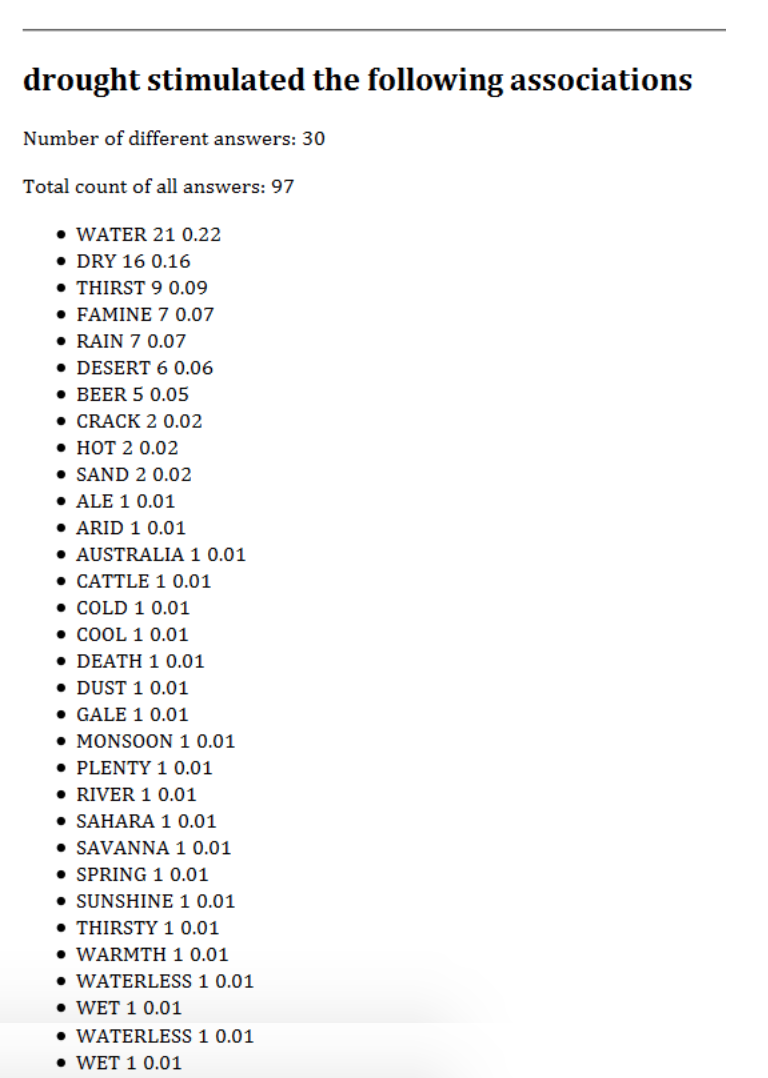
\includegraphics[width=7cm]{img/4_drought_EAT}
  \end{column}
    \hspace{-180pt}
    \begin{column}{10cm}
      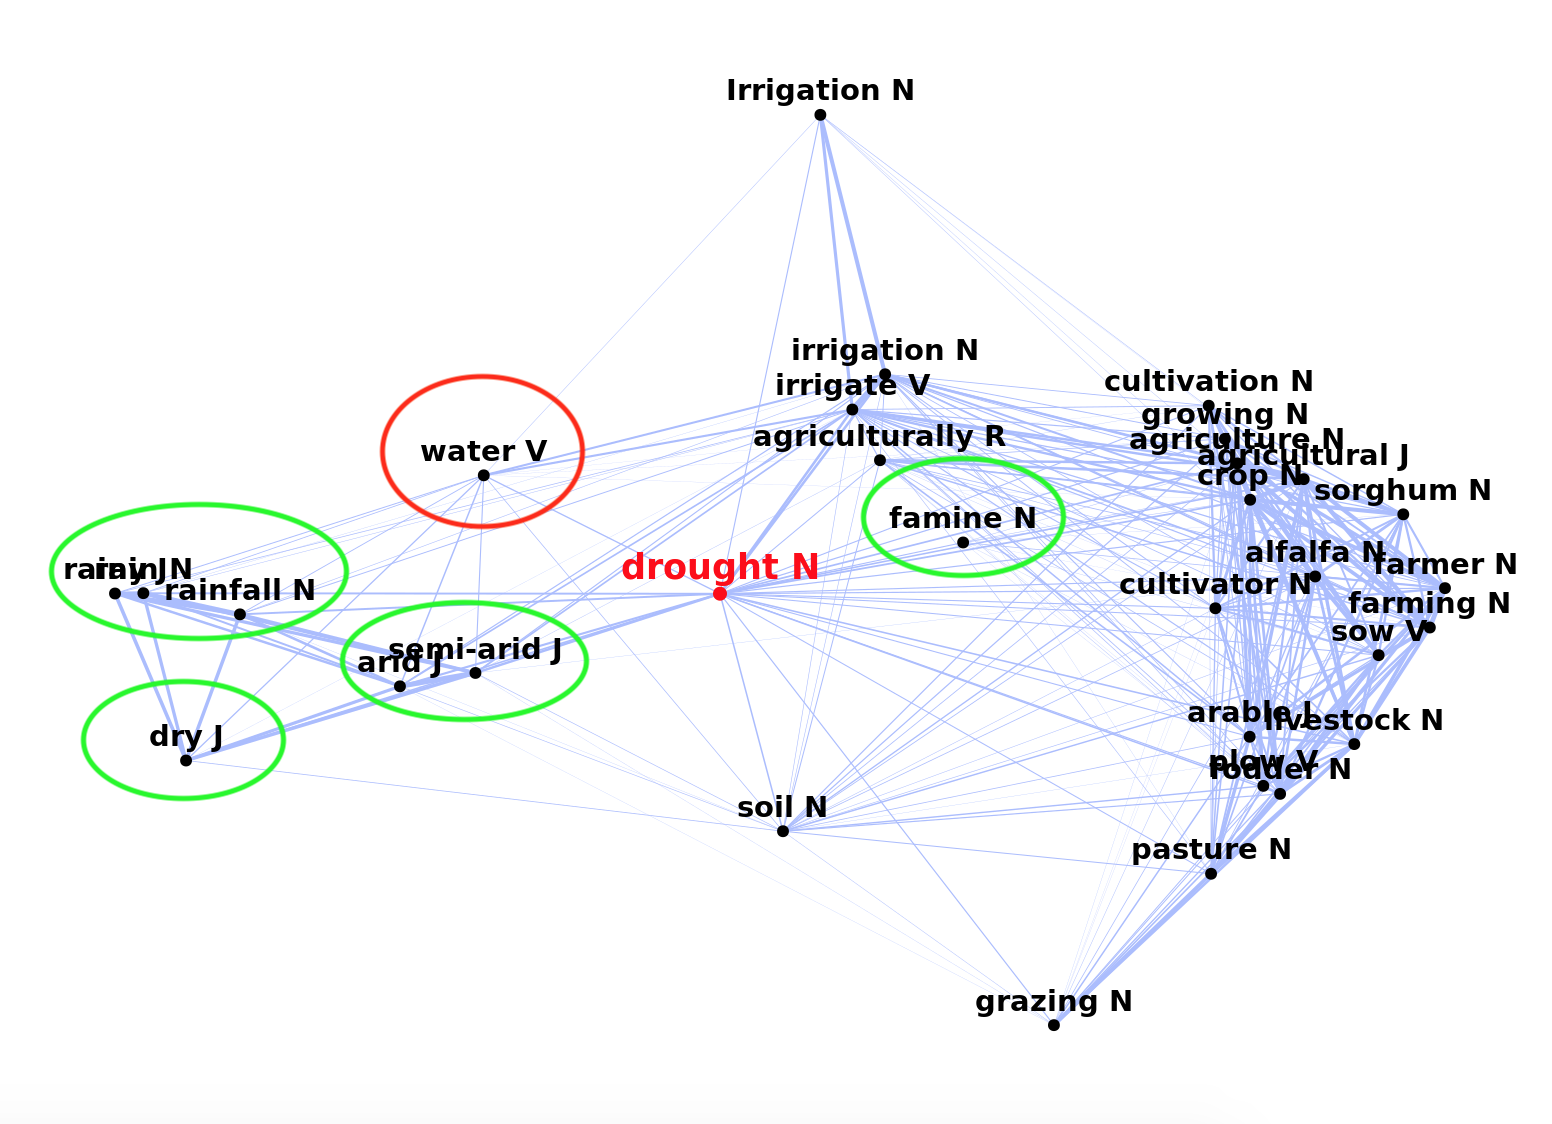
\includegraphics[width=9cm]{img/4_drought_map}
    \end{column}
  \end{columns}
\end{frame}


\begin{frame}
  \frametitle{Free associations \& co-occurrence data}
  \framesubtitle{Previous work}

  \begin{itemize}
  \item \citet{Wettler:Rapp:Sedlmeier:05}
    \begin{itemize} 
    \item Data: subset of EAT (100 stimuli)
    \item Task: prediction of the most common free associate 
    \item Model: \secondary{first-order model}, BNC, large window (20 words)
    \item Result: human associative responses can be predicted from contiguities between words in language use (collocations)
    \end{itemize}
    \gap
  \item ESSLLI 2008 Shared Task
    \begin{itemize} 
    \item Data: subset of EAT (a different set of 100 stimuli)
    \item Task 1: discrimination btw.\ the most common associate and hapax/random distractors \so multiple choice
    \item Task 2: prediction of the most common free associate
    \item Result: \primary{first-order models} (collocations) are better than \secondary{second-order models} (DSMs)
    \end{itemize}
  \end{itemize}
\end{frame}

%%%%%%%%%%%%%%%%%%%%%%%%%%%%%%%%%%%%%%%%%%
\subsection{FAST: Data set and tasks}

\begin{frame}
  \frametitle{The Free ASsociation Task (FAST) data set}
  \framesubtitle{Preprocessing}

  \begin{enumerate}
  \item Starting point: EAT (8210 stimuli), USF (5019 stimuli)
    \gap
  \item<2-> Out-of-context POS tagging 
    \begin{itemize}
    \item Annotate items in EAT and USF (stimuli and responses) with part of speech information
    \item How? Most frequent POS in Web corpus ENCOW: publicly available 10-billion-word Web corpus \so replicability
    \end{itemize}
    \gap
  \item<3-> Out-of-context lemmatization    
    \begin{itemize}
    \item \code{morpha}, a robust morphological analyzer \url{http://users.sussex.ac.uk/~johnca/morph.html}
    \item lemmatization of unknown words based on POS tag
    \end{itemize}
    \gap
  \item<4-> Annotation with frequency information
    \begin{itemize}
    \item frequency lists from ENCOW (lemmatised with \code{morpha})
    \end{itemize}
 \end{enumerate}
\end{frame}


%\TodoSlide{Explain motivation / goals for our data set and task design (including rationale for lemmatization and POS guessing as a help for more linguistic approaches, but not part of the evaluation) $\to$ Gabriella}

\begin{frame}
  \frametitle{The Free ASsociation Task (FAST) data set}
  \framesubtitle{Item selection}

  For each stimulus in EAT (8210) and USF (5019) select a:
  \begin{itemize}
  \item<2-> \primary{\textsc{first}}: the most common associate response
  \item<3-> \primary{\textsc{hapax}}: a response generated for the target once
    \begin{itemize}
    \item or twice for USF (hapax responses are omitted there)
    \item if several \textsc{hapax} candidates are available, pick the one whose lemma frequency matches most closely that of \textsc{first}
    \end{itemize}	
  \item<4-> \primary{\textsc{random}}, by randomly picking a word which was among the top 25\% associates \textit{of another stimulus} (and produced at least 5 times). If possible: 
    \begin{itemize} 
    \item match lemma frequency of \textsc{random} and \textsc{first}
    \item try to use each \textsc{random} only once
    \end{itemize} 
  \end{itemize}

  \gap[1]
  \light{(multiwords, numbers, closed-class words, and other words that do not occur in ENCOW were discarded)} 
\end{frame}

\begin{frame}
  \frametitle{The FAST data set}
  \framesubtitle{Final data set}


  \begin{itemize}
  \item EAT subset: \h{3836} test items + \hh{3774} training items
  \item USF subset: \h{2359} test items + \hh{2360} training items
  \item Item = (\textsc{stimulus}, \textsc{first}, \textsc{hapax}, \textsc{random})
  \item[]
  \item Each stimulus and candidate response provided as lowercased word form and POS-disambiguated lemma
    \begin{itemize}
    \item[+] ENCOW frequency information
    \item[+] \# test subjects who produced response 
  \end{itemize}
  \item[]
  \item Download: \url{https://osf.io/cd8ar/} \citep{Evert:Lapesa:21}
  \item Included as \code{FAST} in package \code{wordspaceEval}
  \end{itemize}
\end{frame}

\begin{frame}
  \frametitle{The FAST dataset}
  \framesubtitle{The new EAT task isn't perfect either \ldots\ yet}

\begin{itemize}
\item Guessing POS from corpus doesn't always work
  \begin{itemize}
  \item e.g.\ \emph{fit}\VERB[purered] $\to$ \emph{epileptic}\ADJ{}, \emph{aristocracy}\NOUN{} $\to$ \emph{lords}\PN[purered]
  \item but very few lemmatization errors (e.g.\ \emph{daiquiri} $\to$ \emph{daiquirus})
  \item[]
  \end{itemize}
\item<2-> Colloquialisms and British slang
  \begin{itemize}
  \item e.g.\ \emph{bod}\NOUN{} $\to$ \emph{person}\NOUN{} (rare in written corpus)
  \item but Web corpus has Welsh \emph{bod} `to be' mistagged as noun
  \item DSM neighbours: \emph{yn}, \emph{hynny}, \emph{mewn}, \emph{hwn}, \emph{gyfer}, \ldots, {\footnotesize 49.}~\emph{\primary{bloke}}, \emph{\primary{techy}}\NOUN, \emph{nus}, \emph{hon}, \ldots, {\footnotesize 60.}~\emph{\primary{guy}}, \emph{mai}, \emph{\primary{geezer}}, \ldots
  \item another example is \emph{mellow}\ADJ{} $\to$ \emph{yellow}\ADJ{}
  \item[]
  \end{itemize}
\end{itemize}
\end{frame}


\begin{frame}
  \frametitle{The FAST tasks}
  
  Task 1: \h{multiple-choice}
  \begin{itemize}
  \item Given a stimulus and a $<$\textsc{first}, \textsc{hapax}, \textsc{random}$>$ triple, determine which of the three candidates is \textsc{first}. 
    \begin{itemize}
    \item Stimulus:  \textit{accept},   $<$  \underline{\textit{receive}}, \textit{love}, \textit{soul}$>$
    \end{itemize}
  \item \textbf{Performance}: accuracy
  \item \textbf{Baseline}: 33.3\%
  \end{itemize}	
    
\end{frame}


\begin{frame}
  \frametitle{The FAST tasks}
  
  Task 2: \h{open-vocabulary lexical access}
  \begin{itemize}
  \item Given a stimulus (e.g.,  \textit{accept}), predict \textsc{first} (\textit{receive}) out of a candidate set (all \textsc{first}: USF=1197, EAT=1633)
  \item \textbf{Performance}: two measures
    \begin{itemize} \footnotesize
    \item \h{Soft accuracy}: average over reciprocal rank ($1/r$) of the true \textsc{first} associate, as a percentage. 
      \begin{itemize} 
      \item similar to accuracy of predicting first associate,\\ but awards partial points for almost correct guesses
      \item always $\geq$ top-1 accuracy
      \end{itemize}        
    \item \h{Log rank}: geometric mean of $r$ across all stimuli. 
      \begin{itemize} 
      \item corresponds to average over $\log r$
      \item better differentiation for models that rarely get the correct answer (and hence score low on soft accuracy)
      \end{itemize}        
    \end{itemize}    		   
  \item \textbf{Baselines}
    \begin{itemize} \footnotesize
    \item \textbf{Soft accuracy}: USF=0.64\% and EAT=0.49\%
    \item \textbf{Log rank}: USF=442.0 and EAT=602.4        
    \end{itemize}              
  \end{itemize}
\end{frame}
  

%%%%%%%%%%%%%%%%%%%%%%%%%%%%%%%%%%%%%%%%%%
\subsection{FAST: Experiments}

\begin{frame}
  \frametitle{Experimental setup}

  \ungap[1]
  \begin{itemize}\small
  \item<1-> \textbf{DSMs (\secondary{second-order})}: symmetric span of 2 \vs 10 words, other parameters set according to \citet{Lapesa:Evert:14a}.
    \begin{itemize}\footnotesize
    \item we experiment with Caron $P$ \citep{Bullinaria:Levy:12}
    \item $P = 0$ equalizes contributions of SVD dimensions
    \end{itemize}

  \item<2-> \textbf{Collocations (\secondary{first-order})}: symmetric span, 2 \vs 10 words,
    with four different association measures \citep{Evert:08}
    \begin{itemize}\footnotesize
    \item conditional probability $P(w_2|w_1)$
    \item log-likelihood $\log G^2$ (popular for collocations)
    \item MI$^2$ = $\log_2 \frac{O^2}{E}$ = geometric mean of $P(w_2|w_1)$ and $P(w_1|w_2)$
    \item PPMI (popular for DSMs)
    \end{itemize}
    
  \item<3-> \textbf{Corpus data}: for DSMs and collocations
    \begin{itemize}\footnotesize
    \item British National Corpus: 100M words
    \item ENCOW 2014 Web corpus, unique sentences: 8.5G words
    \end{itemize}
    
  \item<4-> \textbf{Neural embeddings}: pre-trained models
    \begin{itemize}\footnotesize
    \item word2vec \citep{Mikolov:etc:13}: 100G tokens of Google News
    \item GloVe \citep{Pennington:Socher:Manning:14}: 6G tokens Wikipeda + Gigaword
    \item GloVe: 42G tokens Web data (Common Crawl)
    \item FastText \citep{Joulin:etc:17}: 600G tokens Common Crawl
    \end{itemize}
  \end{itemize} 
\end{frame}

\begin{frame}
  \frametitle{Results: Multiple-choice task}

  \ungap[2]
  \begin{columns}[T]
    \begin{column}{6cm}
      \only<beamer:1| handout:0>{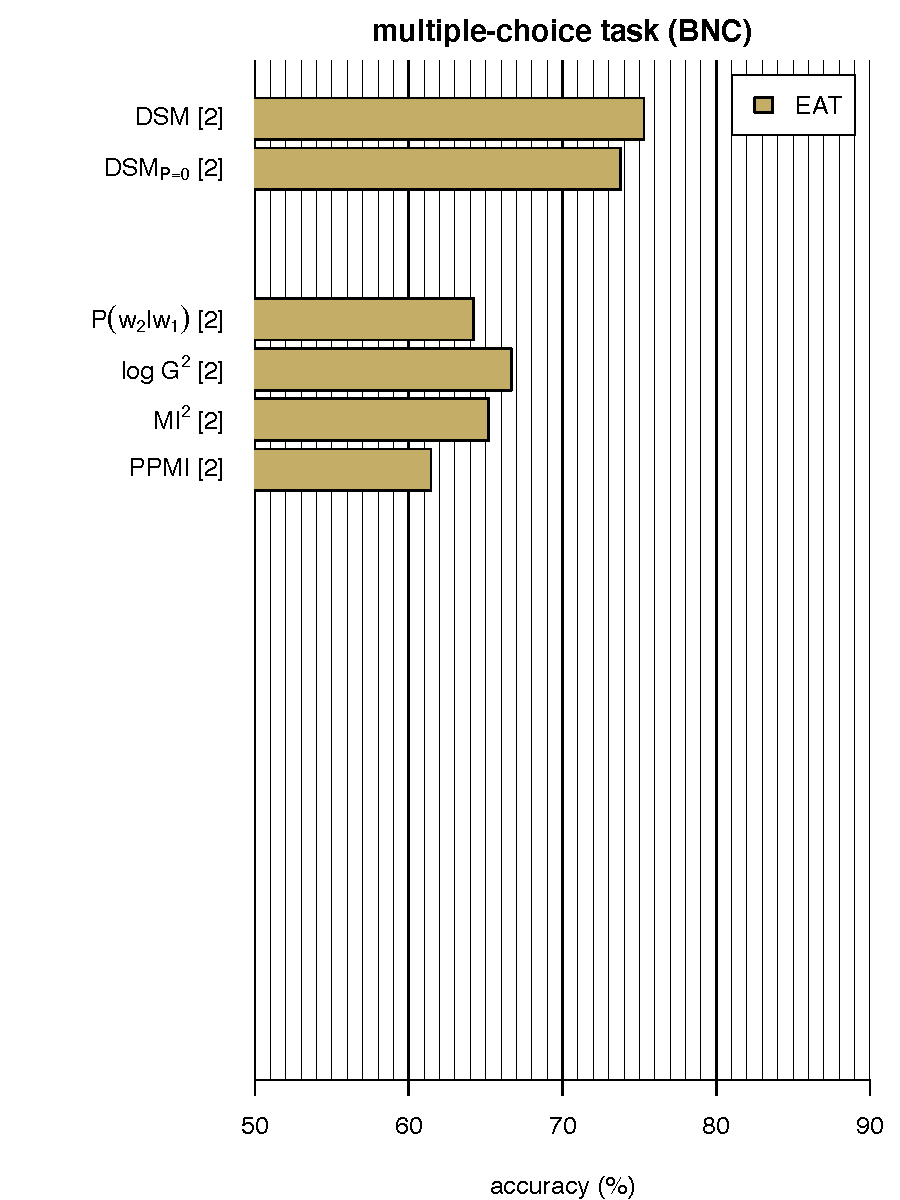
\includegraphics[width=6cm]{img/FAST_task1_BNC_EAT_win2}}%
      \only<beamer:2| handout:0>{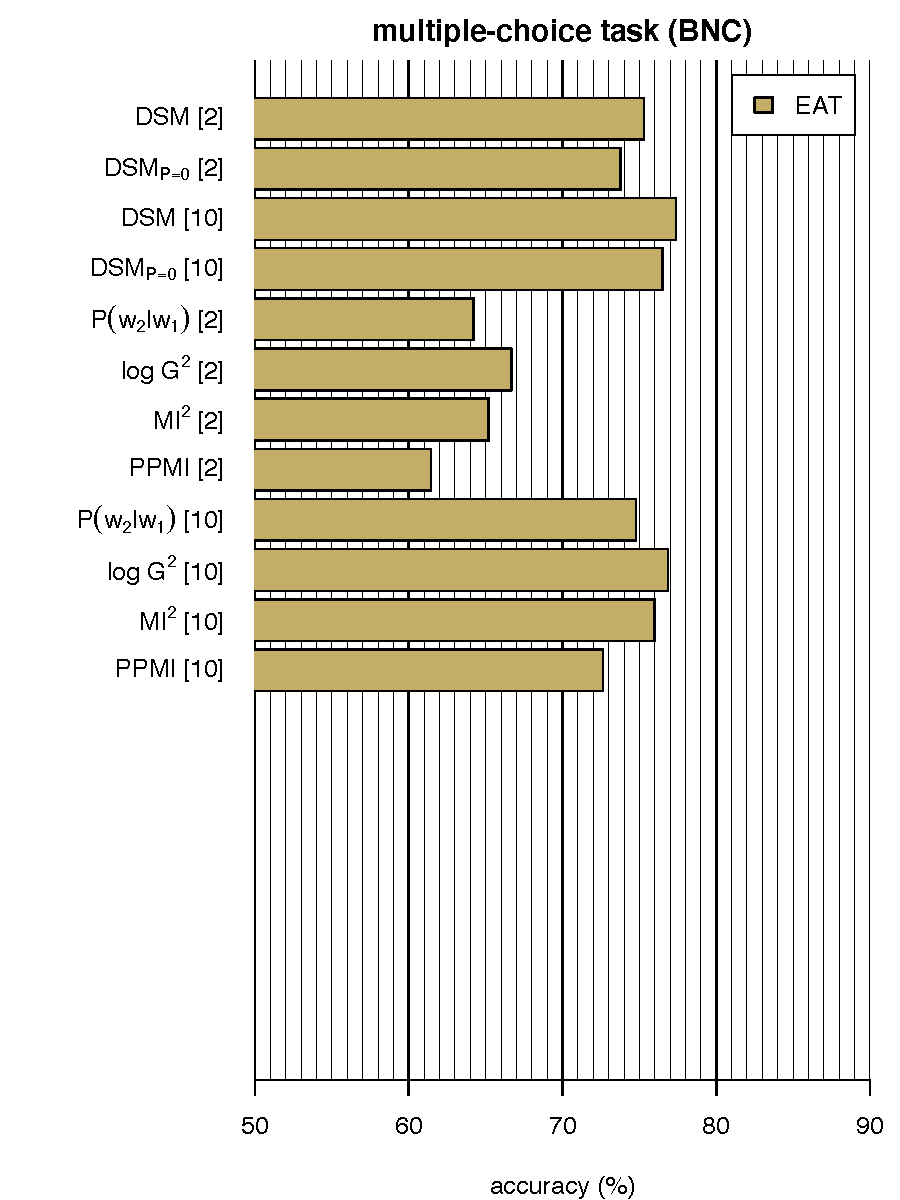
\includegraphics[width=6cm]{img/FAST_task1_BNC_EAT}}%
      \only<beamer:3| handout:1>{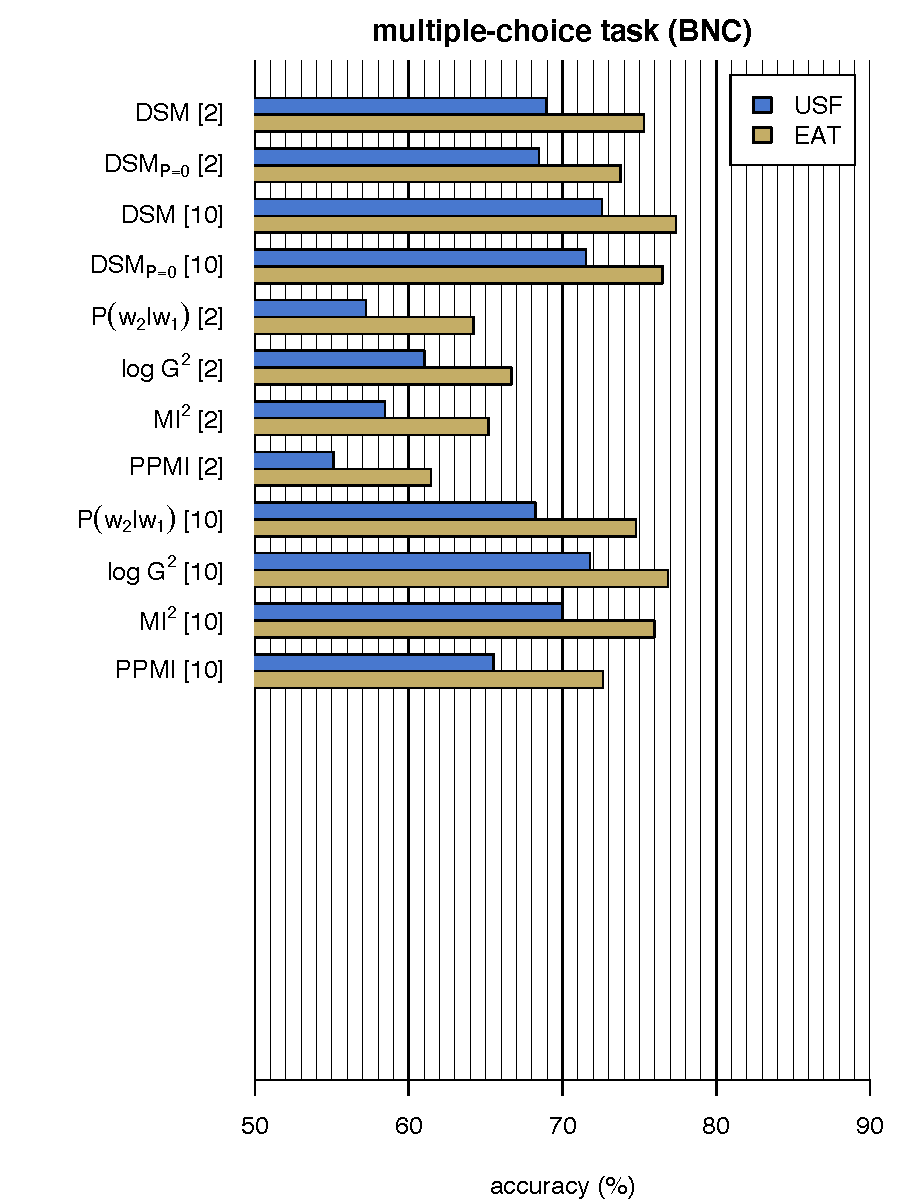
\includegraphics[width=6cm]{img/FAST_task1_BNC}}% 
   \end{column}
    \begin{column}{5cm}
      \begin{itemize}
      \item British National Corpus\\ (100M words)
      \item \only<beamer:1-2| handout:0>{EAT subset}\only<beamer:3>{EAT \vs USF}
      \end{itemize}
    \end{column}
  \end{columns}
\end{frame}

\begin{frame}
  \frametitle{Results: Multiple-choice task}

  \ungap[2]
  \begin{columns}[T]
    \begin{column}{6cm}
      \only<beamer:1| handout:0>{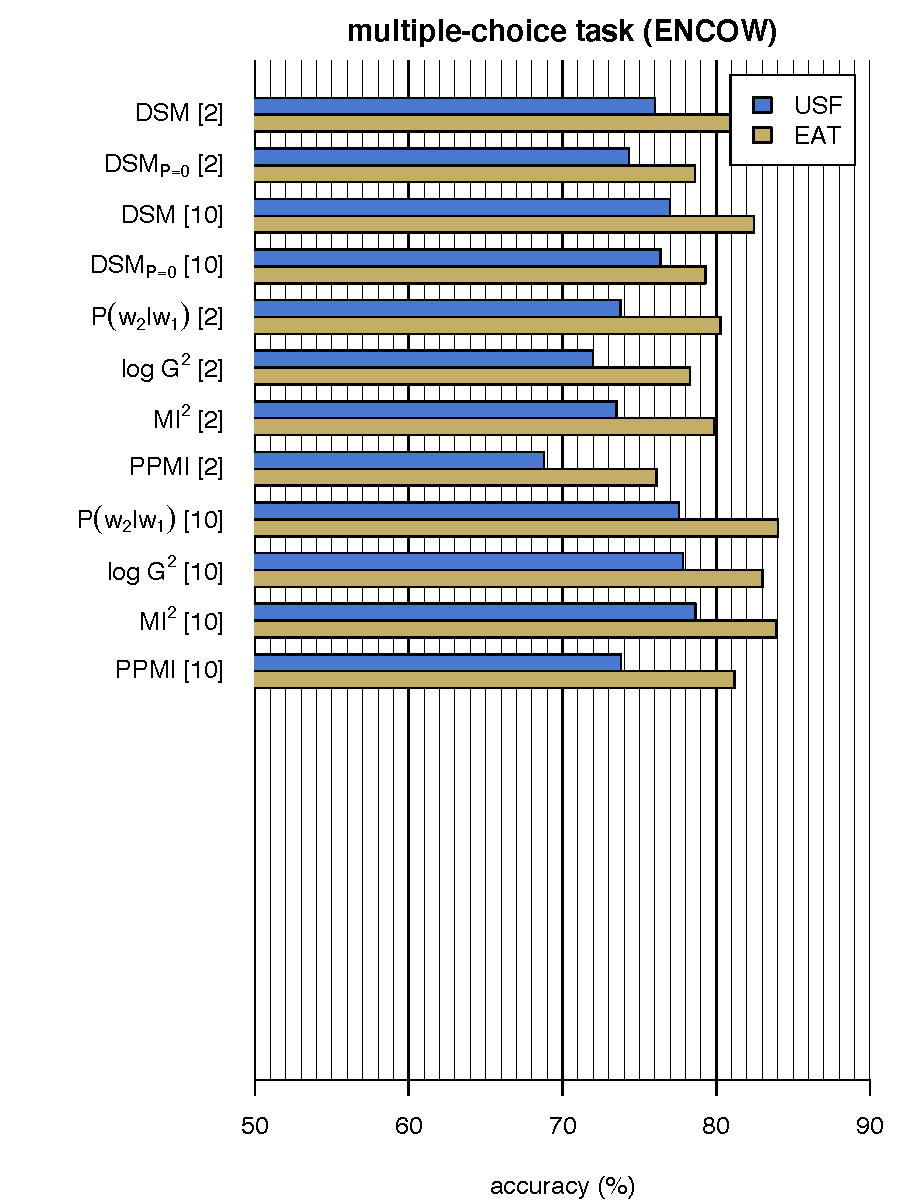
\includegraphics[width=6cm]{img/FAST_task1_ENCOW}}%
      \only<beamer:2-3| handout:0>{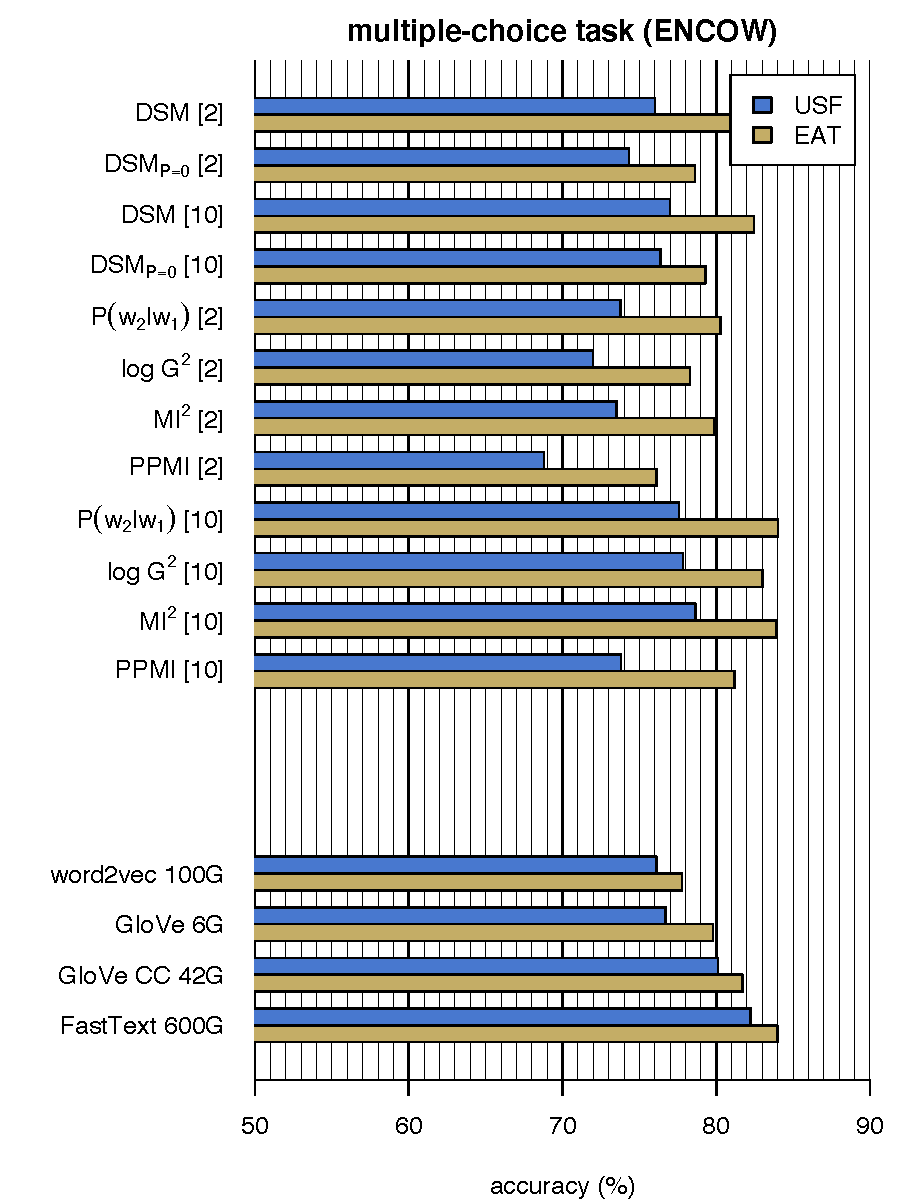
\includegraphics[width=6cm]{img/FAST_task1_ENCOW_embed}}%
      \only<beamer:4| handout:1>{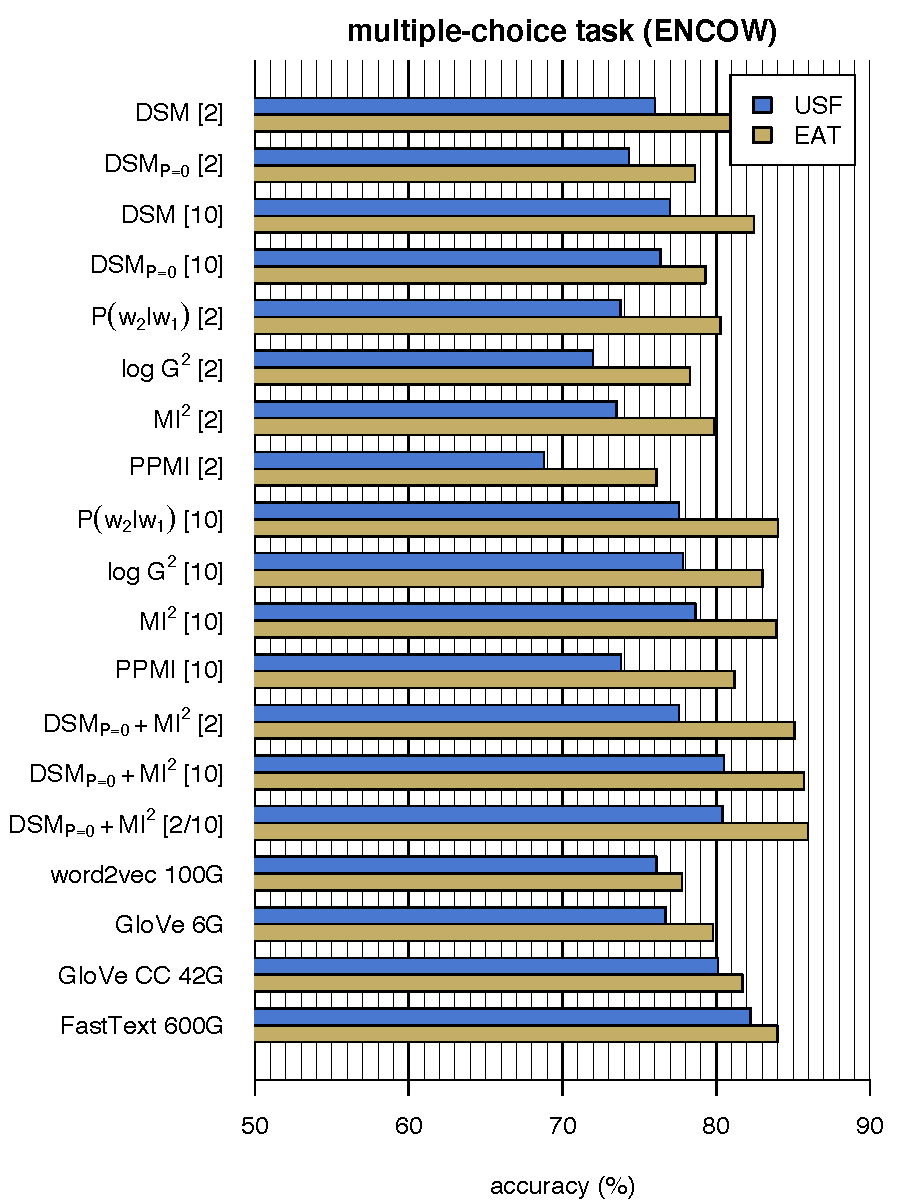
\includegraphics[width=6cm]{img/FAST_task1_ENCOW_all}}%
    \end{column}
    \begin{column}{5cm}
      \begin{itemize}
      \item ENCOW 2014 Web\\ (8.5G words)
      \item EAT \vs USF
      \item<2-> Embeddings trained on much larger corpora
      \item<3-> Combined \First-/\Second-order
        \begin{itemize}
        \item DSM$_{P=0}$ + MI$^2$
        \item using neighbour rank
        \item harmonic mean
        \item<4-> \primary{competitive with state-of-the-art embeddings}
        \end{itemize}
      \end{itemize}
    \end{column}
  \end{columns}
\end{frame}

\begin{frame}
  \frametitle{Results: Multiple-choice task}

  \ungap[2]
  \begin{columns}[T]
    \begin{column}{6cm}
      \footnotesize
      \begin{tabular}{l@{}r|r|r}
        && \secondary{\scriptsize $n = 2359$} & \secondary{\scriptsize $n = 3836$} \\
        model & span & USF & EAT \\
        \hline\hline
        DSM          & 2  & 76.01\% & 81.78\% \\
        DSM$_{P=0}$  & 2  & 74.31\% & 78.62\% \\
        DSM          & 10 & \primary{76.98\%} & \primary{82.46\%} \\
        DSM$_{P=0}$  & 10 & 76.39\% & 79.30\% \\
        \hline
        $P(w_2|w_1)$ & 10 & 77.58\% & \primary{84.02\%} \\
        $\log G^2$   & 10 & 77.83\% & 83.00\% \\
        MI$^2$       & 2  & \primary{78.64\%} & 83.92\% \\
        PPMI         & 10 & 73.80\% & 81.18\% \\
        \hline\hline
        Combined     & 2  & 77.58\% & 85.09\% \\
        Combined     & 10 & \primary{80.50\%} & 85.71\% \\
        Combined     & mix& 80.41\% & \primary{85.97\%} \\
        \hline\hline  
        word2vec     & -- & 76.11\% & 77.78\% \\
        GloVe        & -- & 76.71\% & 79.80\%  \\
        GloVe CC     & -- & 80.12\% & 81.72\%  \\
        FastText     & -- & \primary{82.24\%} & \primary{83.97\%} \\
        \hline\hline
      \end{tabular}
    \end{column}  
    \begin{column}{5cm}
      \begin{itemize}
      \item ENCOW 2014 Web\\ (8.5G words)
      \item EAT \vs USF
      \item Embeddings trained on much larger corpora
      \item Combined \First-/\Second-order
        \begin{itemize}
        \item DSM$_{P=0}$ + MI$^2$
        \item using neighbour rank
        \item harmonic mean
        \item \primary{competitive with state-of-the-art embeddings}
        \end{itemize}
      \end{itemize}
    \end{column}
  \end{columns}
\end{frame}


\begin{frame}
  \frametitle{Results: Open-choice task}

  \ungap[1]
  \footnotesize\centering
  \begin{tabular}{l@{}r|rr|rr}
    && \multicolumn{2}{c|}{\scriptsize $n = 2359$} & \multicolumn{2}{c}{\scriptsize $n = 3836$} \\
    &  & \multicolumn{2}{c|}{USF} & \multicolumn{2}{c}{EAT} \\
    model & span & soft acc. & lrank & soft acc. & lrank \\
    \hline\hline
    DSM          & 2  & 41.54\% &  6.6 & 34.53\% &  9.9 \\
    DSM$_{P=0}$  & 2  & 42.12\% &  7.6 & 34.67\% & 12.1 \\
    DSM          & 10 & 42.01\% &  \primary{6.0} & \primary{35.93\%} &  \primary{9.1} \\
    DSM$_{P=0}$  & 10 & \primary{42.86\%} &  7.1 & 35.68\% & 11.6 \\
    \hline
    \visible<2->{%
    $P(w_2|w_1)$ & 10 & 22.34\% & 17.0 & 11.27\% & 27.1 \\
    $\log G^2$   & 10 & 37.63\% &  6.6 & \primary{34.13\%} &  8.8 \\
    MI$^2$       & 10 & \primary{39.73\%} &  \primary{6.2} & 34.01\% &  \primary{8.7} \\
    PPMI         & 10 & 35.34\% &  8.2 & 29.29\% & 12.2 \\
    \hline\hline}%
    \visible<3->{%
    Combined     & 2  & 42.29\% &  5.5 & 37.54\% &  7.0 \\
    Combined     & 10 & 44.99\% &  4.8 & 39.48\% &  6.5 \\
    Combined     & mix& \primary{45.36\%} & \primary{4.8} & \primary{39.48\%} &  \primary{6.4} \\
    \hline\hline}%
    \visible<4->{%
    word2vec     & -- & 38.98\% &  7.7 & 30.51\% &  14.8 \\
    GloVe        & -- & 39.22\% &  7.6 & 30.19\% &  13.8 \\
    GloVe CC     & -- & 44.01\% &  5.7 & 34.26\% &  10.5 \\
    FastText     & -- & \primary{51.00\%} &  \primary{4.1} & \primary{40.34\%} &   \primary{7.2} \\
    \hline\hline}
  \end{tabular}
\end{frame}



%%%%%%%%%%%%%%%%%%%%%%%%%%%%%%%%%%%%%%%%%%
\subsection{Hands-on exercises}

\begin{frame}
  \frametitle{Hands-on exercise}

  \ungap[1]
  \begin{itemize}
  \item Solve the FAST multiple-choice task with a DSM
    \begin{itemize}
    \item \code{eval.multiple.choice()} does most of the work for you
    \item use \code{details=TRUE} to inspect biggest mistakes and explore performance (e.g.\ wrt.\ frequency of stimulus and response)
    \end{itemize}
    \gap
  \item Can you also make use of first-order (collocation) data?
    \begin{itemize}
    \item hint: the DSM matrix $\mathbf{M}$ contains co-occurrence counts
    \end{itemize}
    \gap
  \item Advanced: Can you combine DSMs with first-order data?
    \begin{itemize}
    \item hint: use average of DSM and first-order ``neighbour'' rank
    \end{itemize}
    \gap
  \item Advanced: Try to solve the open-choice lexical access task
    \begin{itemize}
    \item no ready-made evaluation function in \code{wordspace} yet
    \end{itemize}
    \gap
  \item R code in \code{hands\_on\_part4_fast.R} will help you get started!
  \end{itemize}
\end{frame}

\begin{frame}
  \frametitle{Bonus task: Reverse free associations}
  \framesubtitle{The CogALex-IV shared task \citep{Rapp:14}}

  \ungap[1]
  \begin{block}{Reverse multiword free association}
    \begin{itemize}
    \item wheel, driver, bus, drive, lorry $\rightarrow$ ? 
    \item away, minded, gone, present, ill $\rightarrow$ ?
    \end{itemize}
  \end{block}
  
  \begin{itemize}
  \item Data: subset of EAT (2000 stimuli each training/test)
  \item<2-> Very challenging (best: 35\% accuracy)
    \begin{itemize}
    \item open-ended vocabulary (including inflected surface forms!) 
    \item need for integrating predictions of different stimuli
    \end{itemize}	
  \item<2-> And the winner was \ldots
    \begin{itemize}
    \item a system using first-order statistics to re-rank the output of a ``standard'' DSM \citep{Ghosh:Jain:Paul:14}
	\item our submission: best \First-order: 27.7\% / best \Second-order:  14.0\%
    \end{itemize}
  \item<2-> Try it yourself: \href{http://www.collocations.de/data/CogALex4.rda}{\secondary{\code{CogALex4.rda}}}
  \end{itemize}
\end{frame}

\begin{frame}
  \frametitle{It is practice session time!}
  
  \hspace*{-25pt}
  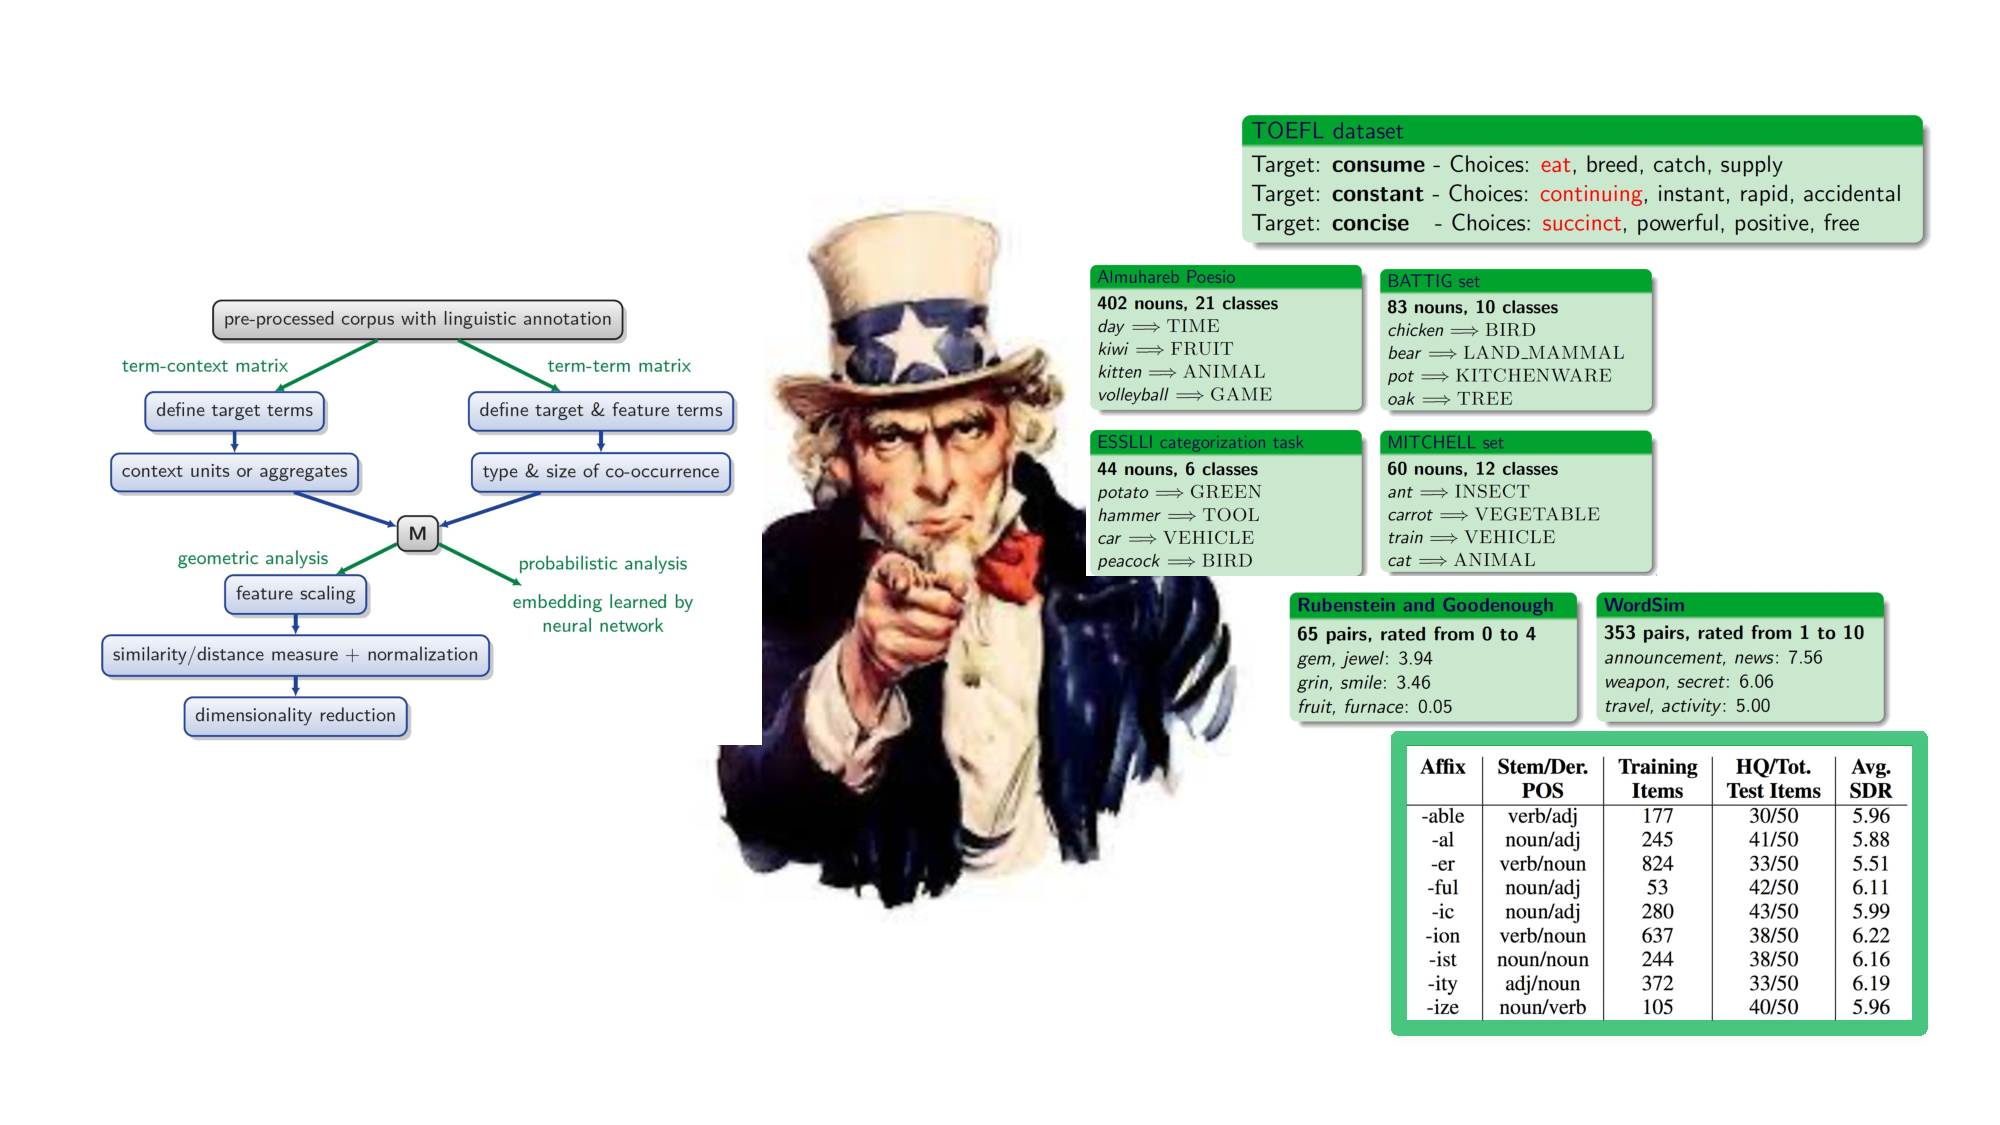
\includegraphics[scale=.35]{img/4_eval_laz}
\end{frame}

%%%%%%%%%%%%%%%%%%%%%%%%%%%%%%%%%%%%%%%%%%%%%%%%%%%%%%%%%%%%%%%%%%%%%% 
%% References (if any)

\frame[allowframebreaks]{
\frametitle{References}
\bibliographystyle{natbib-stefan}
\begin{scriptsize}
  \bibliography{dsm}
\end{scriptsize}
}

\end{document}
